\documentclass[12pt]{report}
%\renewcommand\thesection{\thechapter.\arabic{section}}
%\setcounter{chapter}{0} % Start chapter numbering from 1
% Remove chapter number from section numbering

\usepackage{titlesec} % For customizing section numbering
\usepackage{amsmath} % For enhanced math support
\usepackage{amssymb} % For additional symbols

\usepackage{xcolor} % For custom colors

% Custom section numbering to exclude chapter numbers
\renewcommand{\thesection}{\arabic{section}}
\renewcommand{\thesubsection}{\thesection.\arabic{subsection}}
\renewcommand{\thesubsubsection}{\thesubsection.\arabic{subsubsection}}

% Ensure subsubsections are included in the table of contents
\setcounter{secnumdepth}{3}
\setcounter{tocdepth}{3}


\usepackage[left=2cm,right=2cm,top=2cm,bottom=1.5cm]{geometry}
\usepackage{graphicx}
\usepackage{amsmath}
\usepackage{enumitem}
\usepackage{float} % Include this in your preamble
\graphicspath{{}}

\title{Robotics Project Report}
\author{BAKEL BAKEL}
\date{November, 2024}

\begin{document}
	

	\begin{figure}[H]
		\centering
		
\includegraphics[scale=1.3]{logo} % Adjust the file path and scale as needed
		% Add a label for referencing this figure
	\end{figure}
	\begin{center}
	\fontsize{16}{20}\selectfont\textbf{Erasmus Mundus Joint Master Degree Programme \\[0.5cm]
			in Sustainable Ship and Shipping 4.0}
	\end{center}
	\begin{figure}[H]
		\centering
		
\includegraphics[scale=0.8]{Unina} % Adjust the file path and scale as needed
		% Add a label for referencing this figure
	\end{figure}

	\begin{center}
		\fontsize{16}{20}\selectfont
		\textbf{University of Naples Federico II} \\[0.5cm]
		\textbf{Robotics Technical Elaborate Report} \\[1cm]
		\textbf{Presented by} \\[0.3cm]
		\textbf{Bakel Bakel Begededum} \\[1cm]
		\textbf{Submitted to} \\[0.3cm]
		\textbf{Prof. Vincenzo Lippiello}
	\end{center}
	
	
\tableofcontents % Optional: to display the table of contents
\listoffigures

	\chapter{Kinematics}
	
Given the SCARA robot manipulator below,\\ 
	\begin{figure}[H]
		\centering
		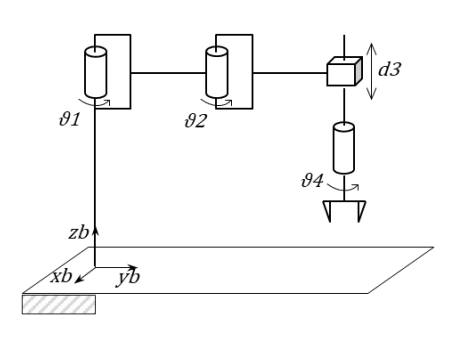
\includegraphics[scale = 1.25]{question} % Adjust the file path and scale as needed
		\caption{Diagram of the Question}
		\label{fig:q} % Add a label for referencing this figure
	\end{figure}

I aim to determine: 
	\begin{enumerate}
		\item The solution to the forward kinematic problem 
		\item The solution to the inverse kinematic problem
		 
	\end{enumerate}
\newpage
\section{Solutions to Kinematic Problems}
	\subsection{Forward Kinematic Problem}
The forward kinematics problem of a robotic system can be addressed through various methodologies and conventions. In this course, the problem was solved with the use of the \textbf{\emph{homogenous transformation matrix}};
	\begin{equation} 
	T^\mathrm{b}_\mathrm{e}(\mathbf{q}) = 
	\begin{bmatrix}
		\mathbf{n}^\mathrm{b}_\mathrm{e}(\mathbf{q}) & \mathbf{s}^\mathrm{b}_\mathrm{e}(\mathbf{q}) & \mathbf{a}^\mathrm{b}_\mathrm{e}(\mathbf{q}) & \mathbf{p}^\mathrm{b}_\mathrm{e}(\mathbf{q}) \\
		0 & 0 & 0 & 1
	\end{bmatrix}
\end{equation}
\\and the \textbf{\emph{Denavit–Hartenberg (D-H) Convention}}, both of which provide systematic frameworks for determining the position and orientation of a robot's end-effector. For this project, I applied all the methods covered in class and extended the scope by incorporating an additional method known as \textbf{\emph{Screw Theory}}, to analyze and solve the forward kinematics. 


By utilizing these methods, the forward kinematic analysis benefits from both systematic parameterization (Homogeneous Matrix and D-H Convention) and advanced geometric interpretation (Screw Theory). This comprehensive approach ensures robustness and flexibility in solving complex robotic configurations.

\subsubsection{Homogeneous Transformation Matrix} This method involves the representation of spatial transformations (rotation and translation) in a unified 4x4 matrix format. Each link and joint of the robot is described by a sequence of transformations, which, when combined, determine the final position and orientation of the end-effector in the base frame.
\\\\Key Features:
\begin{enumerate}
	\item Encodes rotation using a 3x3 rotation matrix.
	\item Encodes translation as a 3x1 vector.
	\item Allows easy composition of transformations using matrix multiplication.
\end{enumerate}
\newpage
{\fontsize{12}{20}\selectfont \textbf{Solution using Homogeneous Transformation Matrix}}
\begin{figure}[H]
	\centering
	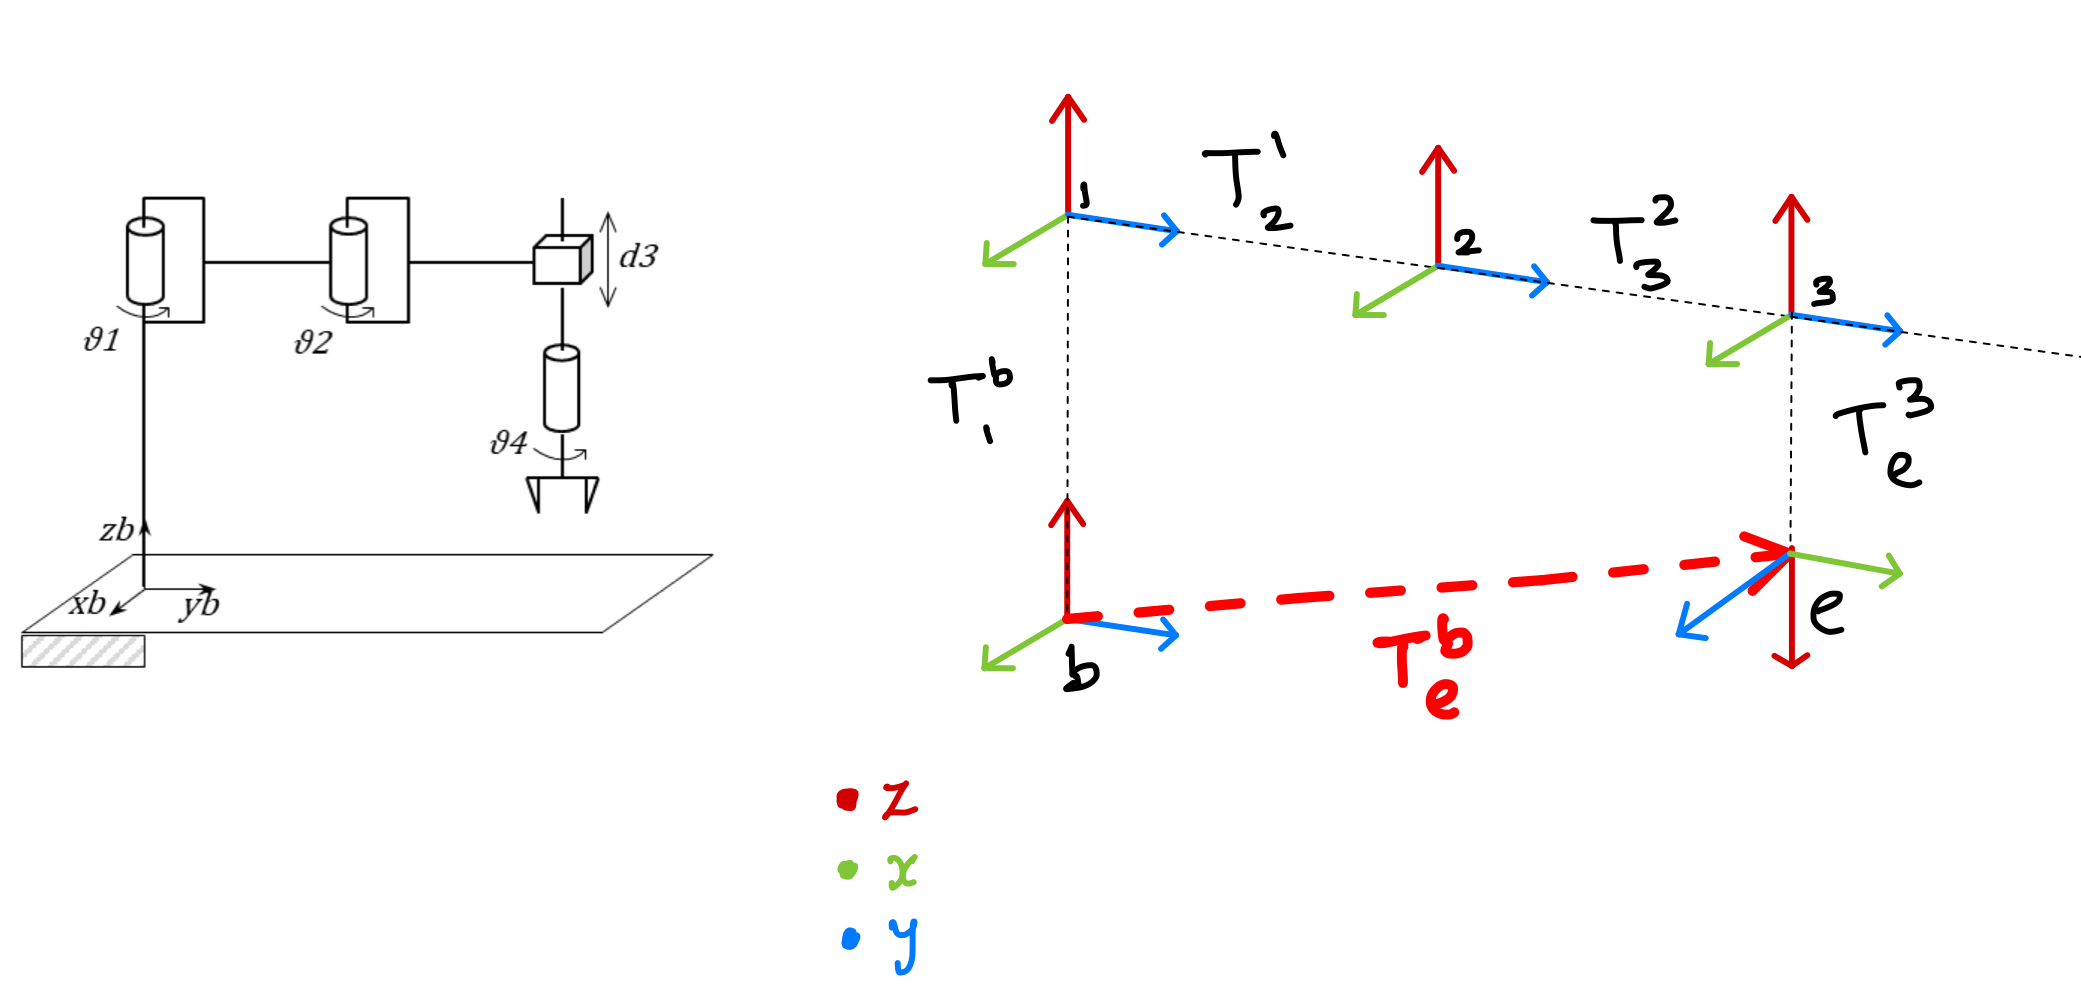
\includegraphics[scale=0.25]{001} % Adjust the file path and scale as needed
	% Add a label for referencing this figure
	\caption{Diagram of Frames of the SCARA Robot}
\end{figure}


Equation 1.2 gives the formula for the forward kinematics of the scara robot as obtained from Figure 2
	\begin{equation} 
	T^b_e = T^b_1\cdot T^1_2\cdot T^2_3\cdot T^3_e 
\end{equation}


\begin{equation}
	T_1^b=\left[\begin{array}{cccc}
		\cos \theta_1 & -\sin \theta_1 & 0 & 0 \\
		\sin \theta_1 & \cos \theta_1 & 0 & 0 \\
		0 & 0 & 1 & d_0 \\
		0 & 0 & 0 & 1
	\end{array}\right]
\end{equation}


\begin{equation}
	T_2^1=\left[\begin{array}{cccc}
			\cos \theta_2 & -\sin \theta_2 & 0 & 0 \\
			\sin \theta_2 & \cos \theta_2 & 0 & a_1 \\
			0 & 0 & 1 & 0 \\
			0 & 0 & 0 & 1
		\end{array}\right]
\end{equation}
\begin{equation}
	\begin{aligned}
		T_3^2=\left[\begin{array}{llll}
			1 & 0 & 0 & 0 \\
			0 & 1 & 0 & a_2 \\
			0 & 0 & 1 & d_3 \\
			0 & 0 & 0 & 1
		\end{array}\right]
	\end{aligned}
\end{equation}
\begin{equation}
	\begin{aligned}
		 T_e^3=\left[\begin{array}{cccc}
			\cos \theta_4 & -\sin \theta_4 & 0 & 0 \\
			\sin \theta_4 & \cos \theta_4 & 0 & 0 \\
			0 & 0 & -1 & 0 \\
			0 & 0 & 0 & 1
		\end{array}\right] 
	\end{aligned}
\end{equation}

Finally, the forward kinematics can be determined by
	\begin{equation} 
	T^b_e = T^b_1\cdot T^1_2\cdot T^2_3\cdot T^3_e 
\end{equation}
Solve this by hand? As an engineer, I will do no such!
I love mathematical rigour but I am an efficient engineer.
I have decided to flex the power of python to solve symbolically the said matrics equation. The \textbf{Sympy} Library was used for this task.\\

\hspace{-20mm} 
	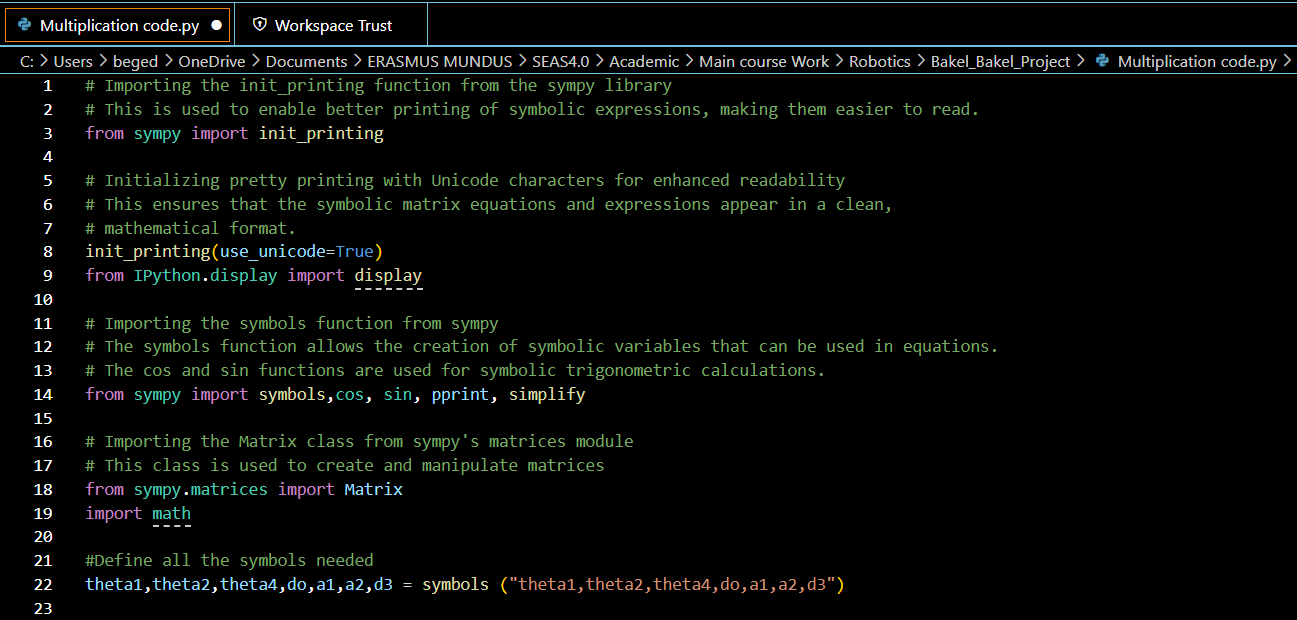
\includegraphics[scale = 0.72]{P1}
	
	\hspace{-20mm} 
	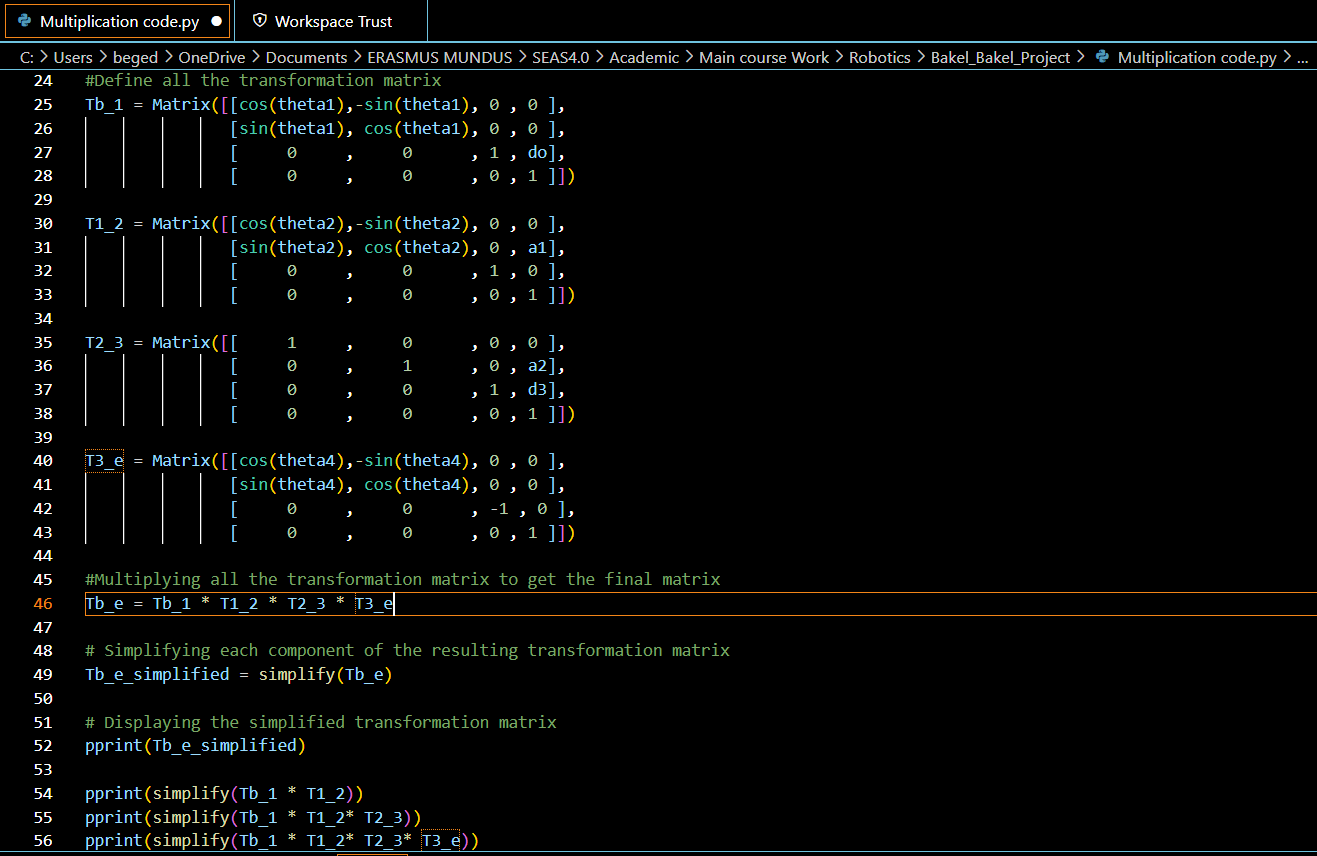
\includegraphics[scale = 0.71]{P2}

Upon running the code, the following matrix was gotten. This is the solution to our forward kinematic problem.

\hspace{-15mm}
\begin{tabular}{cc}
	
\includegraphics[scale=0.3]{voila} & 
	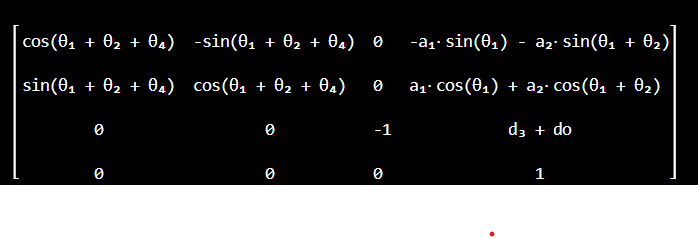
\includegraphics[scale= 1.1]{P3}  \\

\end{tabular}
	\begin{center}

	\textbf{VOILAA!!!}
\end{center}


\subsubsection{Denavit–Hartenberg (D-H) Convention}

This is a standardized convention for modeling the forward kinematics of serial-chain robots. It simplifies the process by defining each joint’s coordinate frame through four parameters: link length, link twist, link offset, and joint angle.\\\\
Key Features:
\begin{enumerate}[label=\roman*.]
	\item Reduces the complexity of defining coordinate systems.
	\item Provides a compact parameterization of the robot's kinematic chain.
	\item Supports systematic derivation of transformation matrices for each joint.\\
\end{enumerate}
a. Firstly, number the joints/points of reference where the frames will be located. 

	\begin{figure}[H]
	\centering
	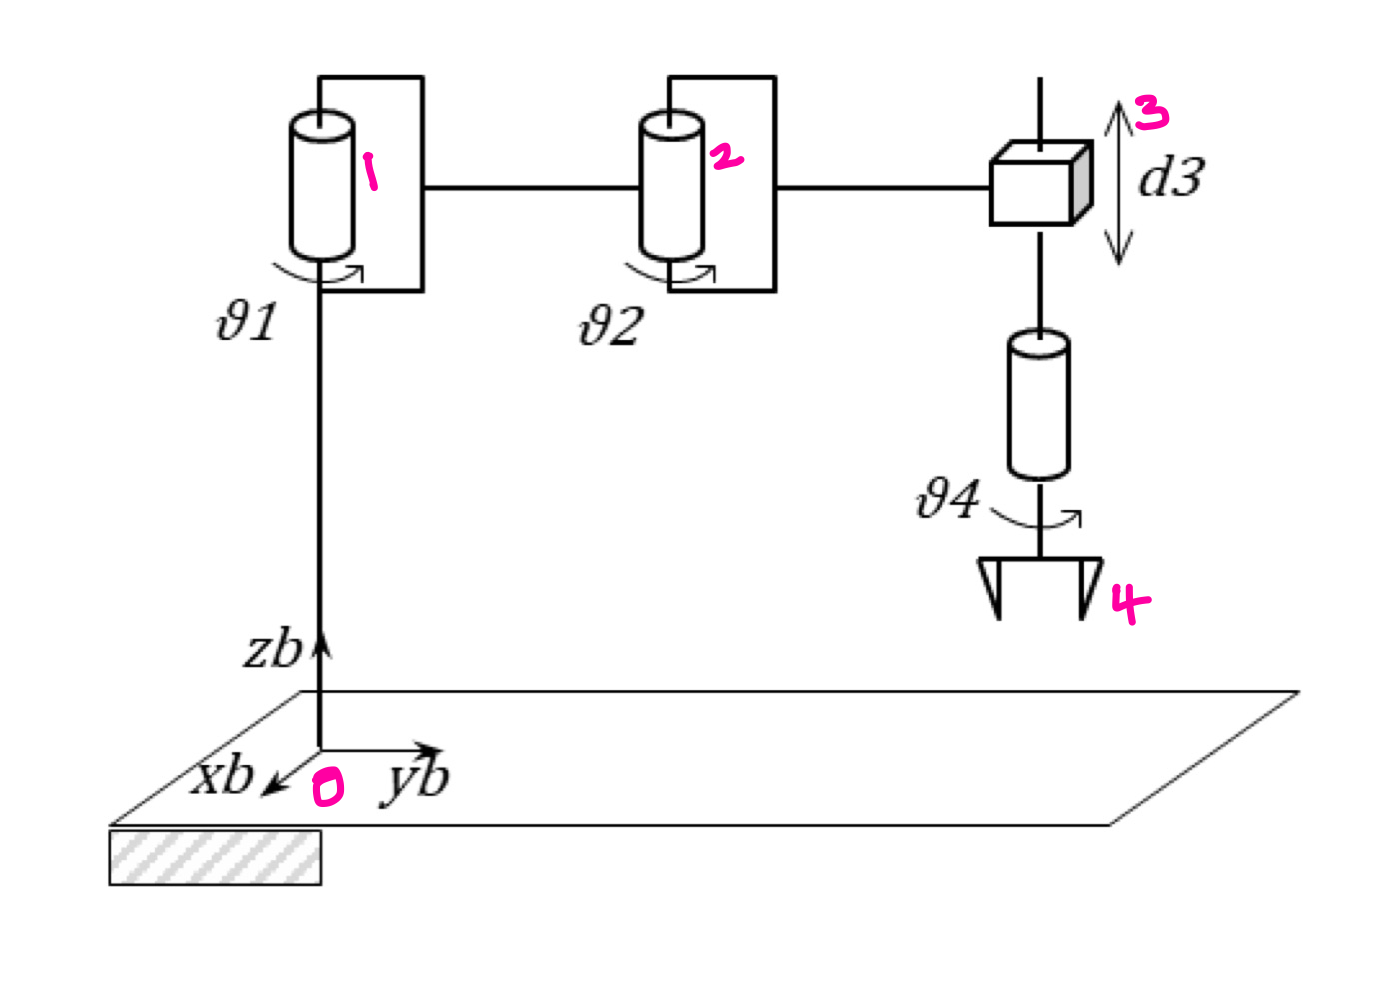
\includegraphics[scale = 0.25]{1} % Adjust the file path and scale as needed
	\caption{Definition of the frames}
	\label{fig:d} % Add a label for referencing this figure
\end{figure}
b. The joint 1 is revolute and following DH Convention, the Z axis will be given as in the image below. The x and y axis of Frame 1 can be obtained correctly as given in the image below.

\begin{figure}[H]
	\centering
	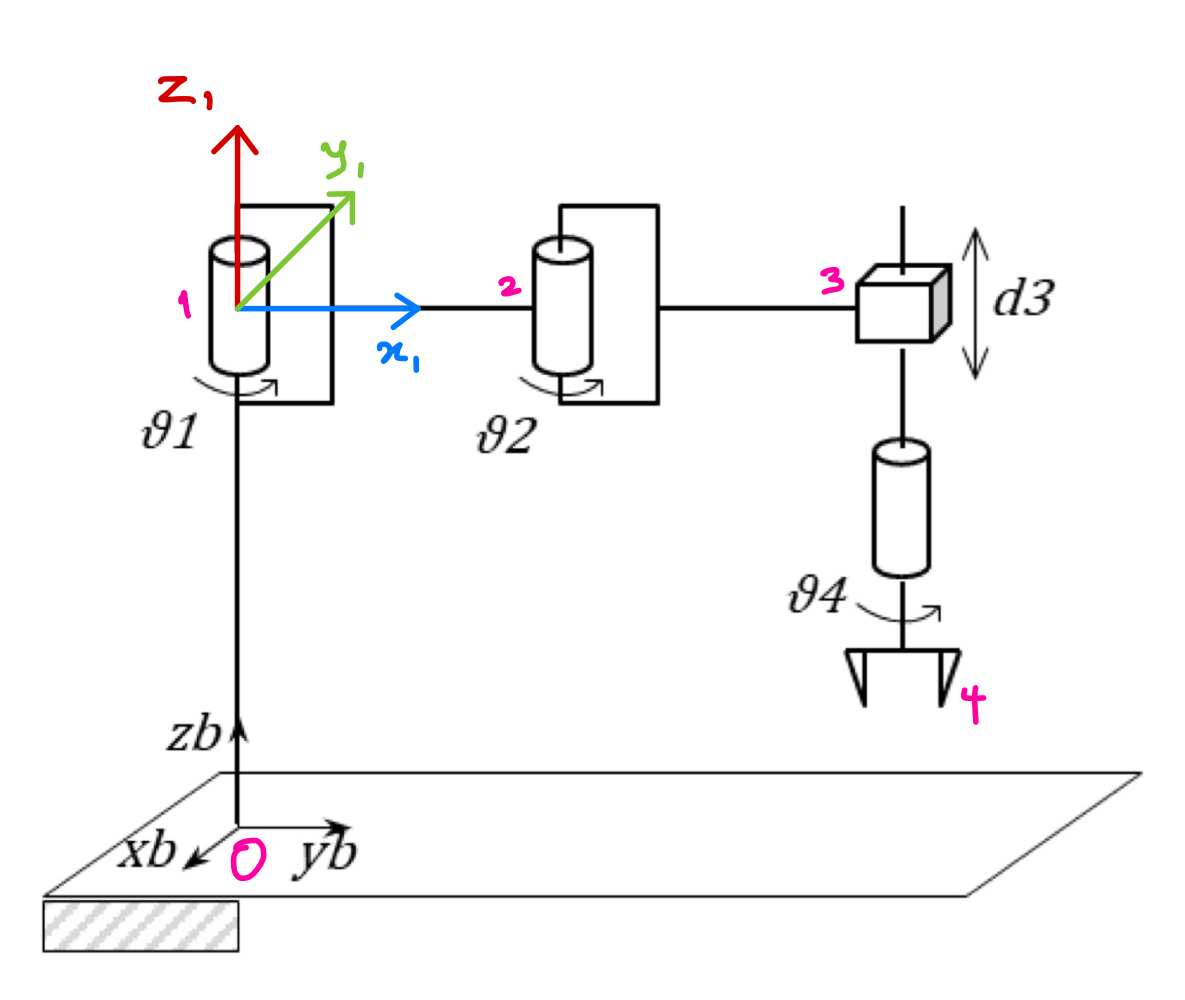
\includegraphics[scale = 0.3]{2} % Adjust the file path and scale as needed
	\caption{Determination of Frame 1}
	\label{fig:your_label} % Add a label for referencing this figure
\end{figure}

c. According to the Denavit-Hartenberg (DH) convention, it is often convenient to align the base frame with Frame 1 for simplicity in deriving the transformation matrices. However, in the context of this problem, the base frame is explicitly defined as part of the problem statement and is distinct from Frame 1.

While I could alter the base frame to match Frame 1 in my solution, this approach is not advisable for practical reasons, especially in an industrial environment:
\begin{enumerate}[label=\roman*.]
	\item Adherence to Given Specifications:
	In real-world engineering problems, the coordinate frames are often pre-defined by the system, client requirements, or the physical environment. Modifying the base frame for convenience could lead to misinterpretations or deviations from the intended design.
	\item Compatibility with Other Systems:
	Industrial setups often involve integration with existing systems or machines. The base frame might be used as a reference for other components, sensors, or control systems. Changing it in calculations could lead to inconsistencies or errors when interpreting results in the actual system.
	
\end{enumerate}
\begin{figure}[H]
	\centering
	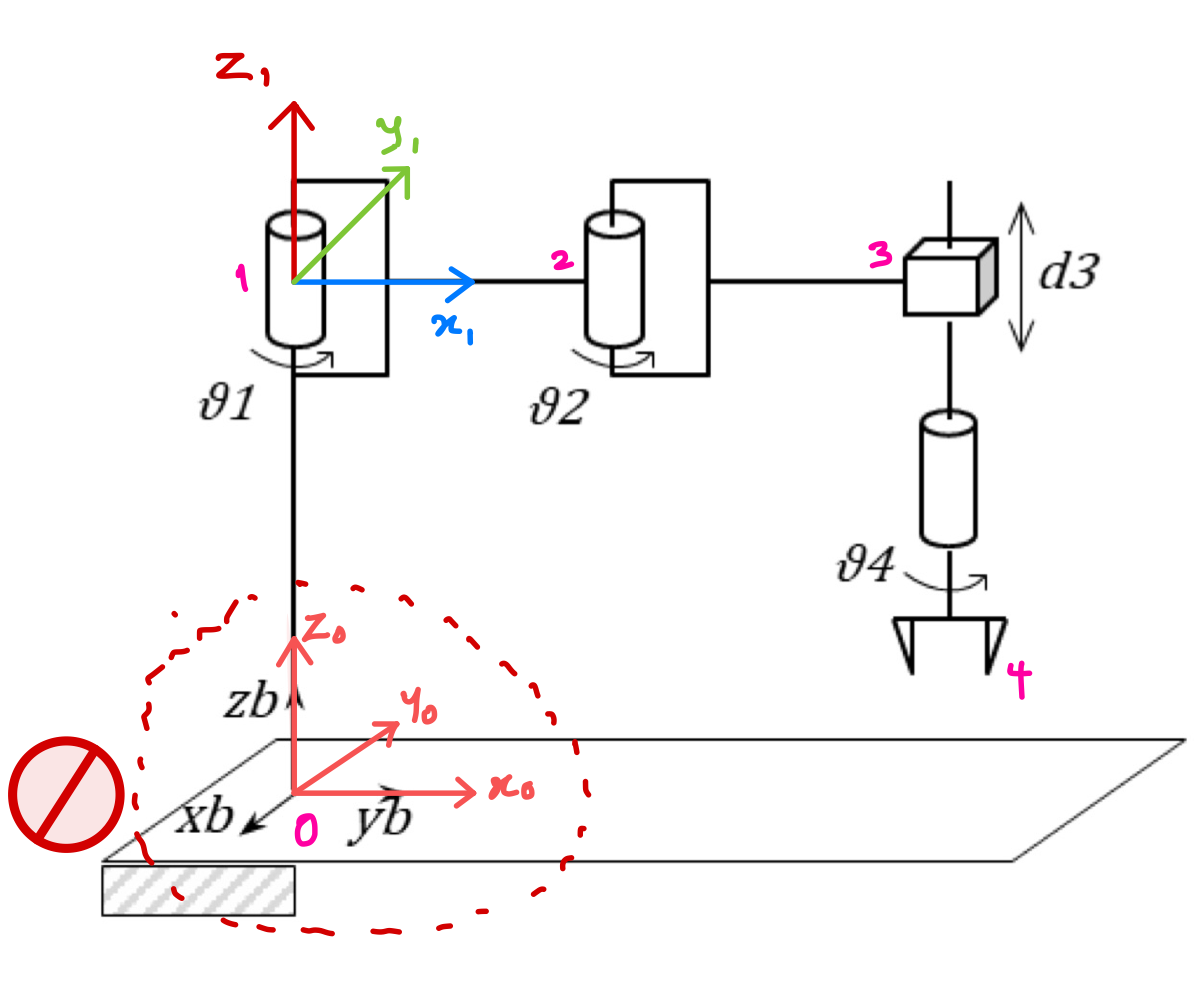
\includegraphics[scale=0.3]{3} % Adjust the file path and scale as needed
	\caption{Illustration of Retaining the Given Base Frame for Consistency with Problem Specifications.}
	\label{fig:retain} % Add a label for referencing this figure
\end{figure}


d. The joint 2 is also revolute so the axis is determined as follows;

\begin{figure}[H]
	\centering
	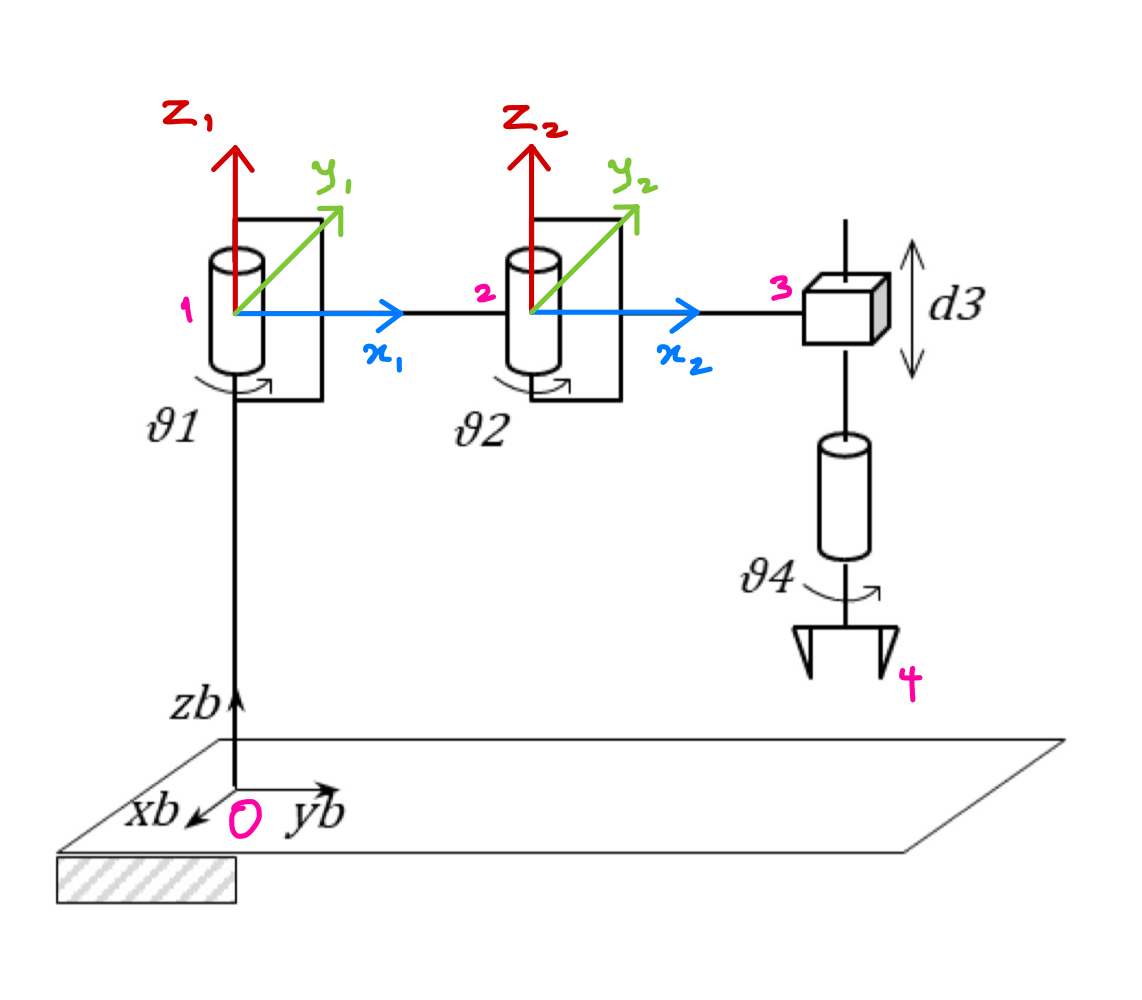
\includegraphics[scale=0.3]{4} % Adjust the file path and scale as needed
	\caption{Determination of Frame 2}
	\label{fig:frame2} % Add a label for referencing this figure
\end{figure}
e. The joint 3 however is a prismatic so the axis is determined as follows;

\begin{figure}[H]
	\centering
	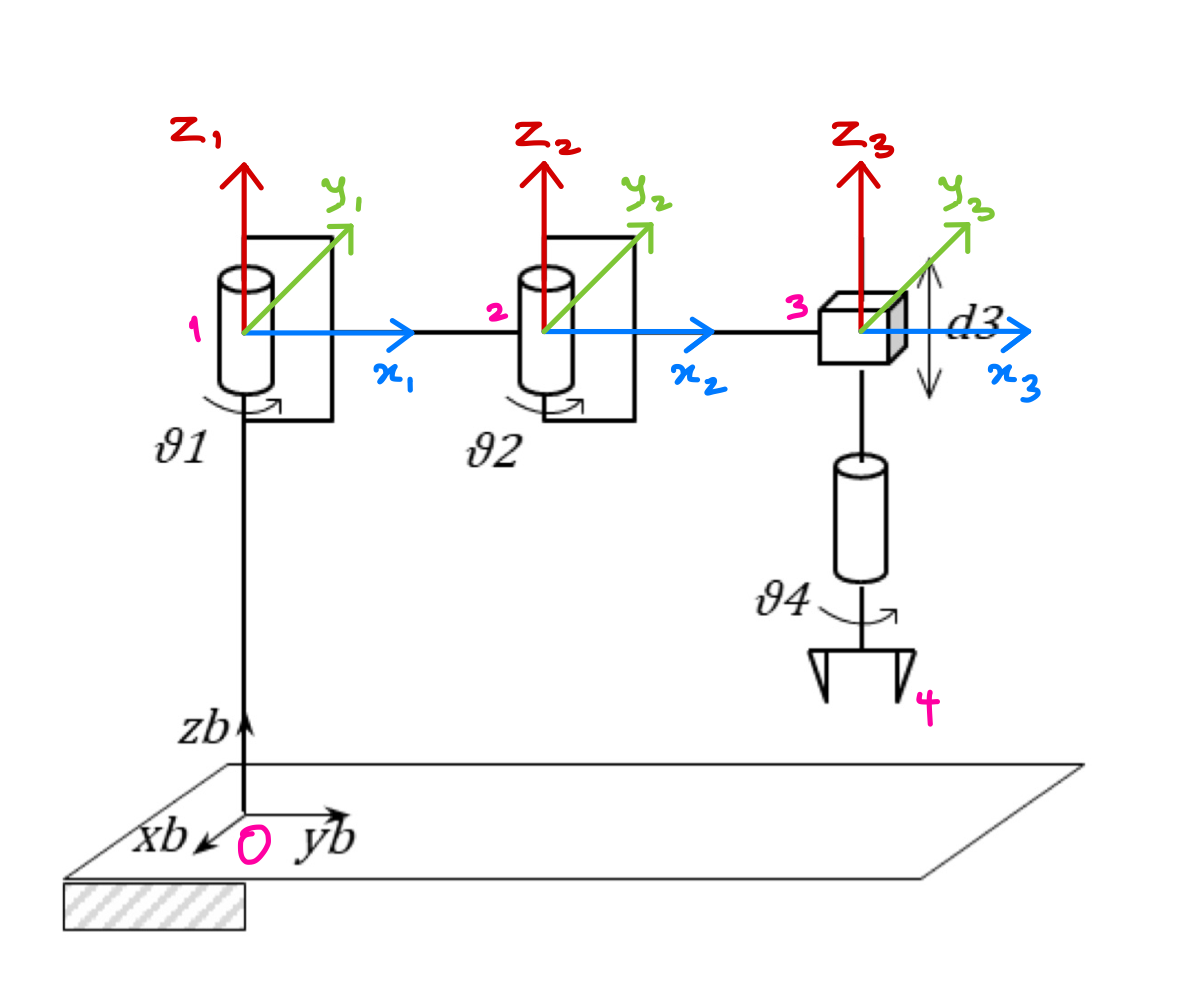
\includegraphics[scale=0.3]{5} % Adjust the file path and scale as needed
	\caption{Determination of Frame 3}
	\label{fig:frame3} % Add a label for referencing this figure
\end{figure}
e. For joint 4, there are some school of thought that insist on putting the frame at the center of the revolute joint and still have a separate frame for the end effector. However, with no clear distance between the joint and the end effector, there is no point in having two separate frames for this configuration and the frame of the revolute joint and the end effector will not only be identical but coincidental.\\

Secondly, from the nature of the question and the position of the end effector, it is intuitive to assign the $(z_4$) facing downwards. But since this doesnt affect much aside our perception of the end effector (which we can easily interpret), I will follow the DH convention that advices the end effector frame to be identical to that of the last frame (Frame 3).

\begin{figure}[H]
	\centering
	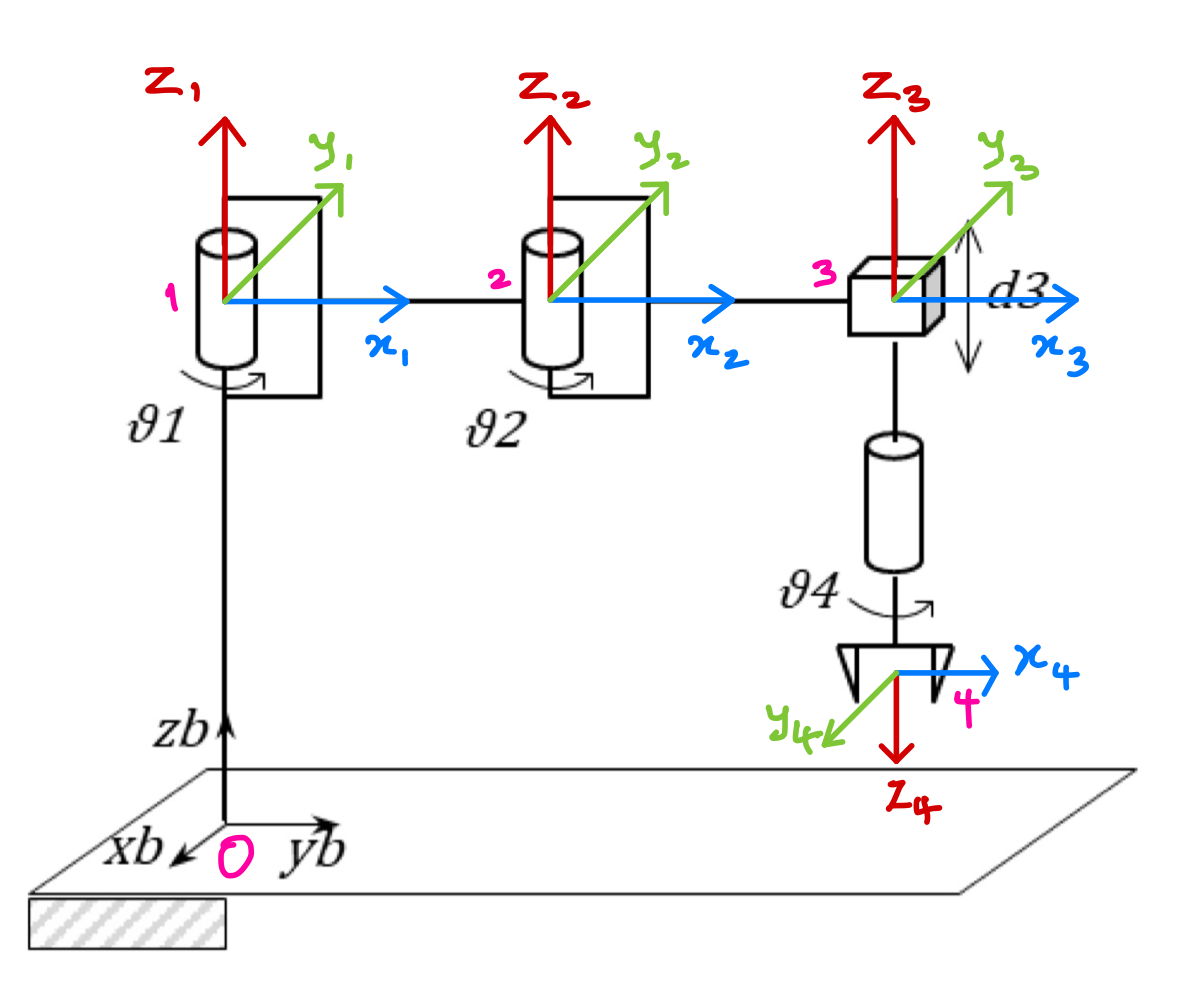
\includegraphics[scale=0.3]{6} % Adjust the file path and scale as needed
	\caption{Schematics showing all the DH Frames of the SCARA robot}
	\label{fig:frame_all} % Add a label for referencing this figure
\end{figure}

\begin{table}[h]
	\centering
	\caption{Table showing DH Parameters}
	\vspace{0.5cm}
	\label{tab:example}
	\begin{tabular}{|c|c|c|c|c|}
		\hline
		
		Link & $a_i$ & $\alpha_i$ & $d_i$ & $\theta_i$ \\
		\hline
		1 & $0_1$ & 0 & $d_0$ & $\frac{\pi}{2}+\theta_1$ \\
		2 & $a_1$ & 0 & 0 & $\theta_2$ \\
		3 & $a_2$ & 0 & 0 & 0 \\
		4 & 0 & $\pi$ & $d_3$ & $\theta_4$ \\
		\hline
	\end{tabular}
	
\end{table}


\subsubsection{Screw Theory}

Screw Theory offers a geometric and algebraic framework to describe motion and kinematics in terms of twists (velocity screws) and wrenches (force screws). It represents the motion of a rigid body as a combination of rotational and translational components about a screw axis.\\\\
Key Features:
\begin{enumerate}[label=\roman*.]
	\item Models motion using Plücker coordinates for lines.
	\item Efficiently handles instantaneous kinematics, including singularities and constraints.
	\item Extends naturally to spatial motion analysis, offering insights into both the kinematic and dynamic aspects of robotic systems.
\end{enumerate}
To find the transformation matrix using screw theory for the SCARA robot, we need to use the following steps:

A screw motion is characterized by:
1. A rotation about an axis (with angular velocity \(\omega\)).
\\2. A translation along the same axis (with linear velocity \(v\)).

The transformation matrix for a rigid body moving under a screw motion is given by:
\begin{equation}
	T = e^{\hat{\xi} \theta}
\end{equation}

where:
\(\hat{\xi}\) is the twist matrix, defined as:
\begin{equation}
	\hat{\xi} =
	\begin{bmatrix}
		\hat{\omega} & v \\
		0 & 0
	\end{bmatrix}
\end{equation}\\\\\(\hat{\omega}\) is the skew-symmetric matrix for angular velocity \(\omega\).
\\ \(v\) is the linear velocity vector.
\\ \(\theta\) is the joint variable (angle or displacement).

\subsubsection*{Step-by-Step Process}
The SCARA robot has the following joints:
\\1. Revolute joint 1 (\(\theta_1\)):
Rotation about the Z-axis at the base.
\\2. Revolute joint 2 (\(\theta_2\)):
Rotation about the Z-axis at the second joint.
\\3. Prismatic joint (\(d_3\)):
Linear motion along the Z-axis.
\\4. Revolute joint 4 (\(\theta_4\)):
Rotation about the Z-axis at the end-effector.
\\\\Define the Twists (\(\xi\))\\
For each joint, we define the twist \(\xi\) as:
\begin{equation*}
	\xi = 
	\begin{bmatrix}
		\omega \\
		v
	\end{bmatrix}
\end{equation*}


Joint 1 (\(\theta_1\)):

\begin{equation}
	\omega_1 = \begin{bmatrix} 0 \\ 0 \\ 1 \end{bmatrix}, \quad
	v_1 = \begin{bmatrix} 0 \\ 0 \\ 0 \end{bmatrix} \quad
	\Rightarrow \quad
	\xi_1 =
	\begin{bmatrix}
		0 \\ 0 \\ 1 \\ 0 \\ 0 \\ 0
	\end{bmatrix}
\end{equation}


Joint 2 (\(\theta_2\)):

\begin{equation}
	\omega_2 = \begin{bmatrix} 0 \\ 0 \\ 1 \end{bmatrix}, \quad
	v_2 = \begin{bmatrix} -a_1 \\ 0 \\ 0 \end{bmatrix} \quad
	\Rightarrow \quad
	\xi_2 =
	\begin{bmatrix}
		0 \\ 0 \\ 1 \\ -a_1 \\ 0 \\ 0
	\end{bmatrix}
\end{equation}


Joint 3 (\(d_3\)):

\begin{equation}
	\omega_3 = \begin{bmatrix} 0 \\ 0 \\ 0 \end{bmatrix}, \quad
	v_3 = \begin{bmatrix} 0 \\ 0 \\ 1 \end{bmatrix} \quad
	\Rightarrow \quad
	\xi_3 =
	\begin{bmatrix}
		0 \\ 0 \\ 0 \\ 0 \\ 0 \\ 1
	\end{bmatrix}
\end{equation}


Joint 4 (\(\theta_4\)):

\begin{equation}
	\omega_4 = \begin{bmatrix} 0 \\ 0 \\ 1 \end{bmatrix}, \quad
	v_4 = \begin{bmatrix} -a_1 - a_2 \\ 0 \\ 0 \end{bmatrix} \quad
	\Rightarrow \quad
	\xi_4 =
	\begin{bmatrix}
		0 \\ 0 \\ 1 \\ -a_1 - a_2 \\ 0 \\ 0
	\end{bmatrix}
\end{equation}


3. Compute the Exponential Map
For each joint, the transformation matrix is given by:
\begin{equation}
	T_i = e^{\hat{\xi}_i \theta_i}
\end{equation}


The twist matrix \(\hat{\xi}\) is:
\begin{equation}
	\hat{\xi} =
	\begin{bmatrix}
		\hat{\omega} & v \\
		0 & 0
	\end{bmatrix}
\end{equation}


For revolute joints (\(\omega \neq 0\)):
\begin{equation}
	\hat{\omega} =
	\begin{bmatrix}
		0 & -\omega_z & \omega_y \\
		\omega_z & 0 & -\omega_x \\
		-\omega_y & \omega_x & 0
	\end{bmatrix}
\end{equation}

For prismatic joints (\(\omega = 0\)):
\begin{equation}
	\hat{\xi} =
	\begin{bmatrix}
		0 & 0 & 0 & v_x \\
		0 & 0 & 0 & v_y \\
		0 & 0 & 0 & v_z \\
		0 & 0 & 0 & 0
	\end{bmatrix}
\end{equation}


4. Final Transformation Matrix
The total transformation matrix \(T_b^e\) is:
\begin{equation}
	T_b^e = T_1 T_2 T_3 T_4
\end{equation}

where:
\begin{equation}
	T_1 = e^{\hat{\xi}_1 \theta_1}
\end{equation}
\begin{equation}
	T_2 = e^{\hat{\xi}_2 \theta_2}
\end{equation}
\begin{equation}
	T_3 = e^{\hat{\xi}_3 d_3}
\end{equation}
\begin{equation}
	T_4 = e^{\hat{\xi}_4 \theta_4}
\end{equation}




\subsubsection{Verification with Corke's Robotics Toolbox}
\begin{figure}[H]
	\centering
	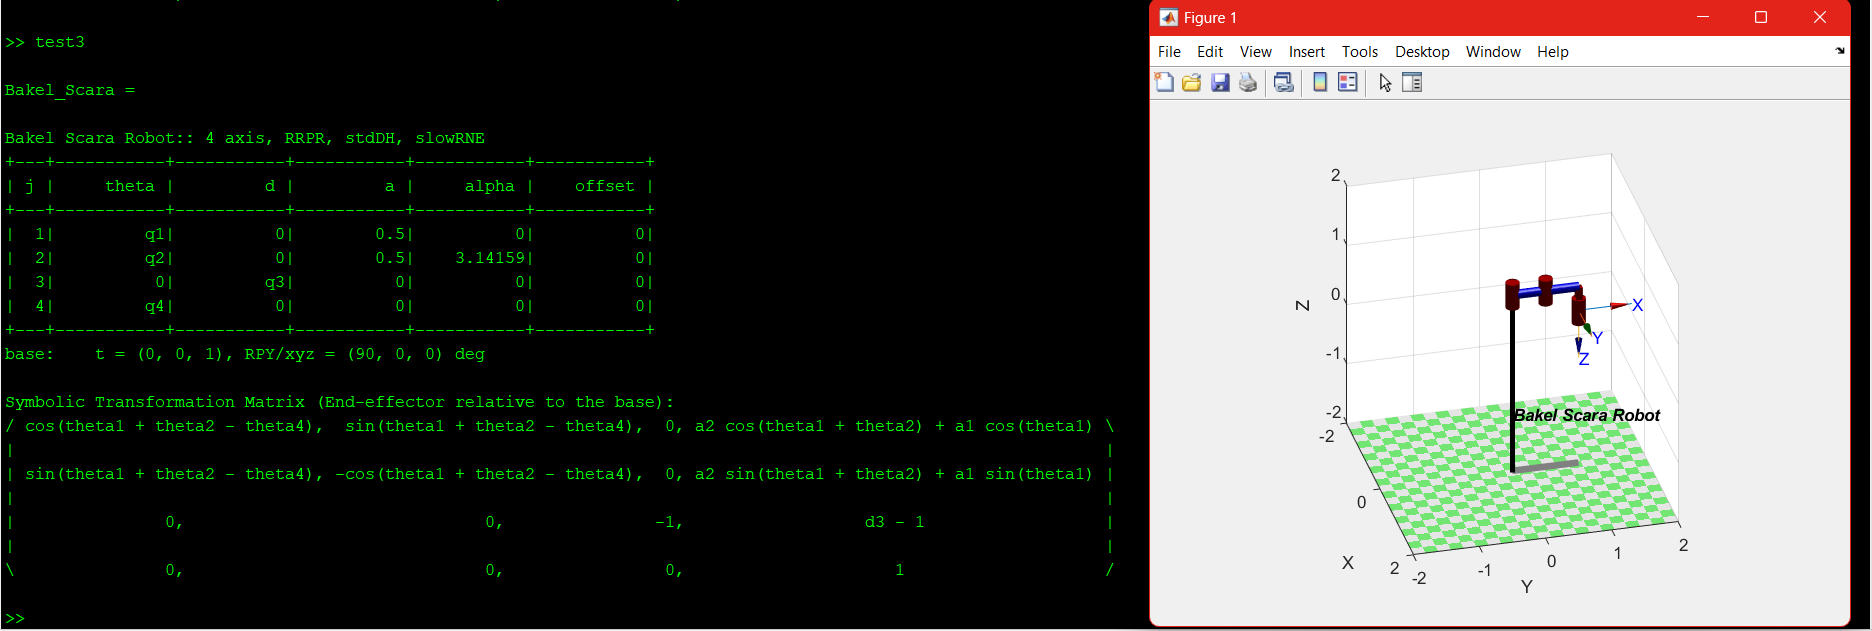
\includegraphics[scale=0.47]{run1} % Adjust the file path and scale as needed
	\caption{Schematics showing all the DH Frames of the SCARA robot}
	\label{fig:run1} % Add a label for referencing this figure
\end{figure}

\begin{figure}[H]
	\centering
	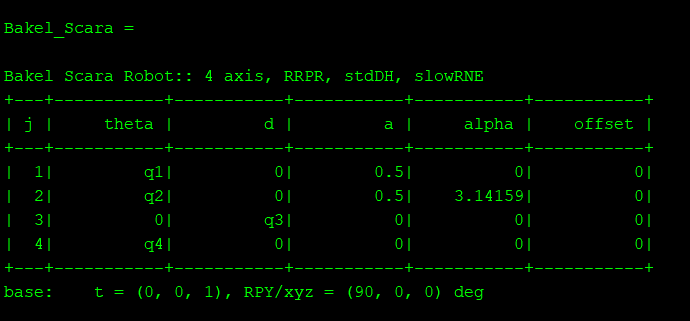
\includegraphics[scale=1.2]{run2} % Adjust the file path and scale as needed
	\caption{Schematics showing DH table of the SCARA robot using joints}
	\label{run2} % Add a label for referencing this figure
\end{figure}

\begin{figure}[H]
	\hspace{-1cm} 
	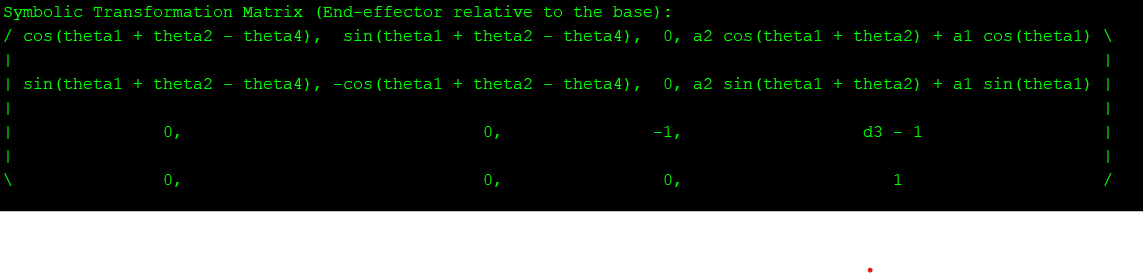
\includegraphics[scale=0.8]{run3} % Adjust the file path and scale as needed
	\caption{The Transformation Matrix}
	\label{run3} % Add a label for referencing this figure
\end{figure}
\begin{figure}[H]
	\centering
	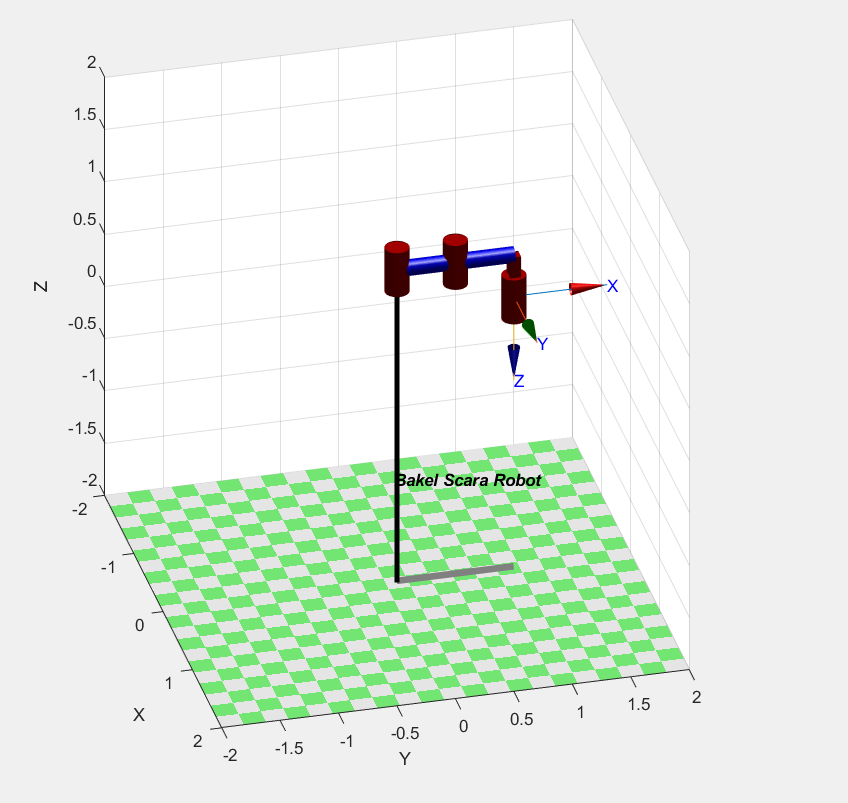
\includegraphics[scale=1]{run4} % Adjust the file path and scale as needed
	\caption{Model of the SCARA robot}
	\label{run4} % Add a label for referencing this figure
\end{figure}
\begin{figure}[H]
	\centering
	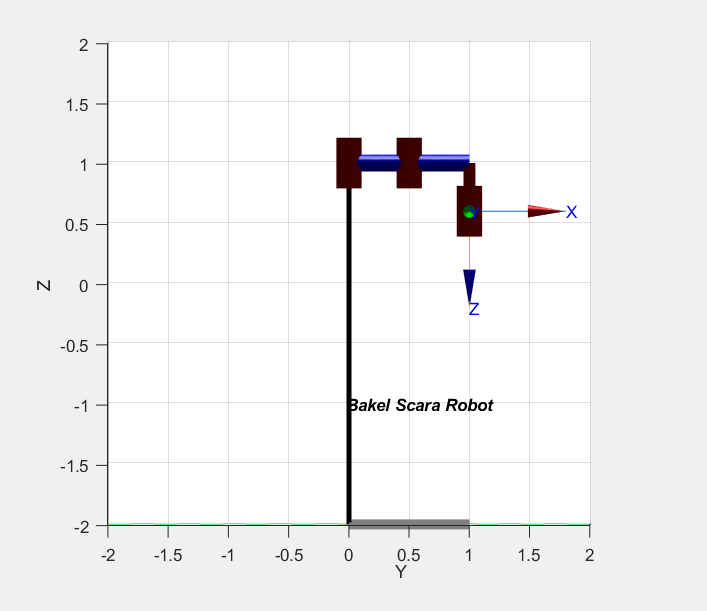
\includegraphics[scale=1]{run5} % Adjust the file path and scale as needed
	\caption{Model of the SCARA robot in ZY Frame}
	\label{run5} % Add a label for referencing this figure
\end{figure}

	\subsection{Inverse Kinematic Problem}
	
	The inverse kinematic problem is formulated as follows: \\\\Given the position and orientation of the end effector, find the joint variables of the robot. \\\\The given SCARA robot has 4 DOF, so for its position and orientation to be fully represented, we need 4 variables which are; x, y, z for position, and \(\psi\) for orientation 
	\begin{equation}
		\psi=\theta_1+\theta_2+\theta_3
	\end{equation}

	\begin{figure}[H]
		\centering
		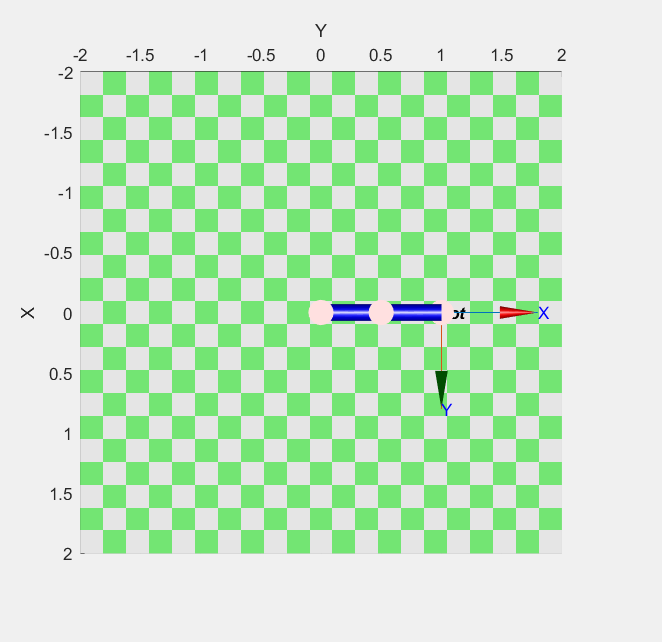
\includegraphics[scale=1]{run7} % Adjust the file path and scale as needed
		\caption{Top View (XY Plane) of the robot}
		\label{run7} % Add a label for referencing this figure
	\end{figure}
		\begin{figure}[H]
		\centering
		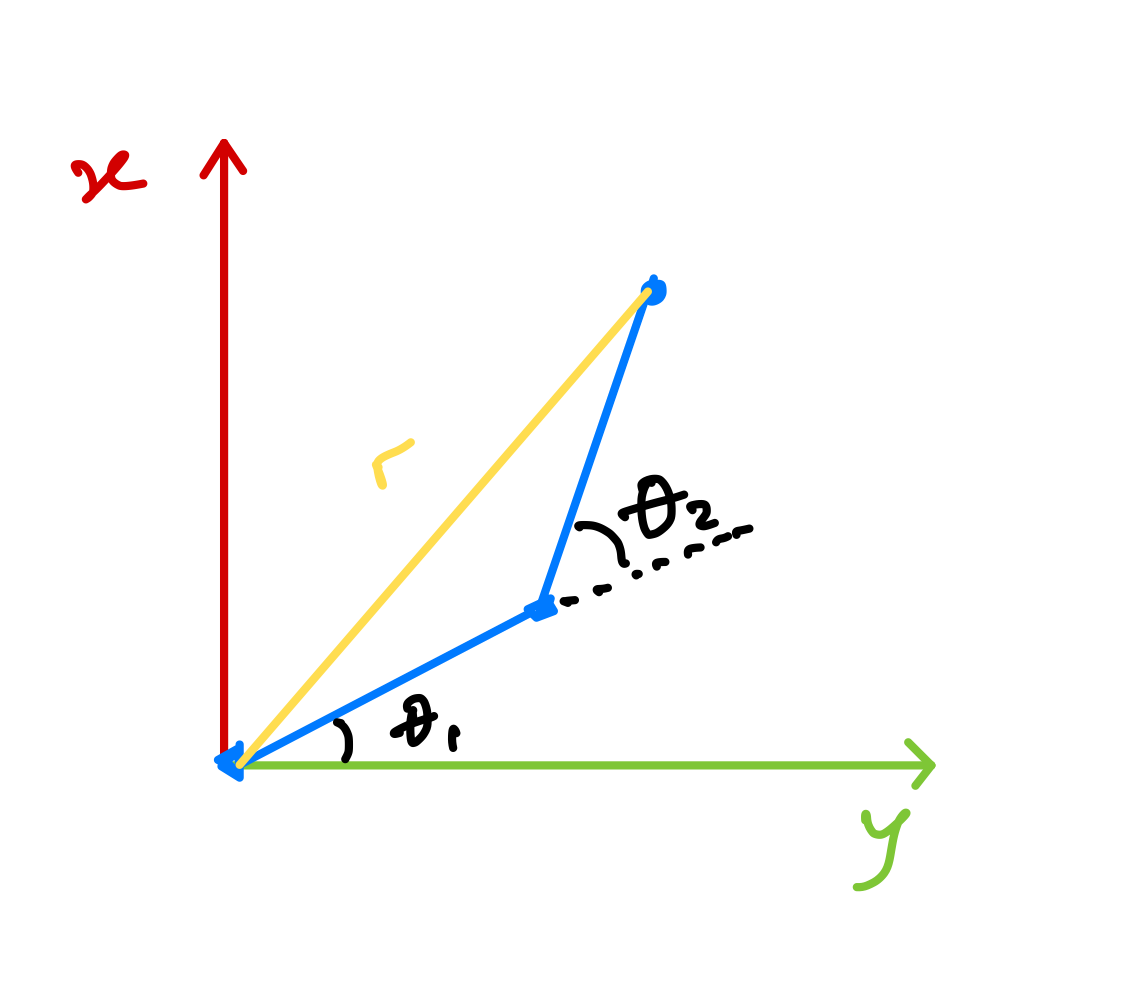
\includegraphics[scale=0.3]{20} % Adjust the file path and scale as needed
		\caption{Top View of the SCARA robot to solve inverse kinematics}
		\label{run7} % Add a label for referencing this figure
	\end{figure}
	\begin{equation}
		\begin{aligned}
			&\text { As } z_2 \text { is along } z_4\\
			&\begin{aligned}
				& p_2\left(x_2, y_2\right) \geq\left(x_1\right) \\
				& r^2=x^2+y^2 \\
				& r^2=a_1^2+a_2^2-2 a_1 a_2 \cos x
			\end{aligned}\\
			&\begin{aligned}
				& 1 \theta_2=\pi-\alpha \\
				& \cos \theta_2=-\cos \alpha \\
				& r^2=a_1^2+a_2^2+2 a_1 a_2 \cos \theta_2 \\
				& \sin ^2 \theta_2+\cos ^2 \theta_2=1 \\
				&  \sin \theta_2=\sqrt{1-\cos ^2 \theta_2} \\
				& \beta=\tan ^{-1} \frac{a_2 \sin \theta_2}{a_1+a_2 \cos _2} \\
				& \gamma=\tan ^{-1} \frac{4}{x} \\
				& \theta_1=\gamma-\frac{\beta}{r} \\
				& \theta_1=\tan ^{-1} \frac{1}{x}-\tan ^{-1} \frac{a_2 \sin \theta_2}{a_1+a_2 \cos \theta_2}
			\end{aligned}
		\end{aligned}
	\end{equation}
		\begin{equation}
		\theta_1 = \tan^{-1}\left(\frac{y}{x}\right) - \tan^{-1}\left(\frac{a_2 \sin \theta_2}{a_1 + a_2 \cos \theta_2}\right)
	\end{equation}
	
	\begin{equation}
		\theta_2 = \cos^{-1}\left(\frac{x^2 + y^2 - \left(a_1^2 + a_2^2\right)}{2 a_1 a_2}\right)
	\end{equation}

\subsubsection{Verification with Corke's Robotics Toolbox}
\begin{figure}[H]
	\centering
	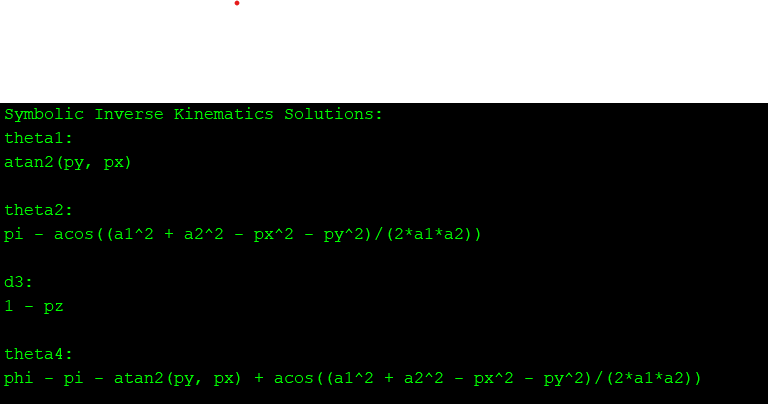
\includegraphics[scale=1]{V1} % Adjust the file path and scale as needed
	\caption{Verification of Inverse Kinematics from Corke's Robotics Toolbox}
	\label{V1} % Add a label for referencing this figure
\end{figure}


	
	\subsection{Representing my end-effector in terms of Euler angles}
It is possible to convert our SCARA 4-DOF configuration and the transformation matrix into Euler angles.

Euler angles describe the orientation of a rigid body (in this case, the end-effector) as a sequence of rotations around different axes. Since the SCARA robot has only 1 rotational DOF (the combined rotation angle), the process simplifies significantly.
\\\\Analyzing the Transformation Matrix:\newline
The transformation matrix you provided is:

$$
T=\left[\begin{array}{cccc}
	\cos \left(\theta_1+\theta_2+\theta_4\right) & -\sin \left(\theta_1+\theta_2+\theta_4\right) & 0 & x \\
	\sin \left(\theta_1+\theta_2+\theta_4\right) & \cos \left(\theta_1+\theta_2+\theta_4\right) & 0 & y \\
	0 & 0 & -1 & z \\
	0 & 0 & 0 & 1
\end{array}\right]
$$

The rotational part (upper-left $3 \times 3$ ) shows the orientation:

$$
R=\left[\begin{array}{ccc}
	\cos \left(\theta_1+\theta_2+\theta_4\right) & -\sin \left(\theta_1+\theta_2+\theta_4\right) & 0 \\
	\sin \left(\theta_1+\theta_2+\theta_4\right) & \cos \left(\theta_1+\theta_2+\theta_4\right) & 0 \\
	0 & 0 & -1
\end{array}\right]
$$

The translational part shows the position:

$$
P=\left[\begin{array}{l}
	x \\
	y \\
	z
\end{array}\right]
$$


Steps to Extract Euler Angles:
1. Choose an Euler Angle Convention:

Euler angles can be defined in different conventions (e.g., ZYX, XYZ). For a SCARA robot, the typical convention is Z-X-Z or Z-Y-Z since rotations occur primarily around the Z-axis.
2. Decompose the Rotation Matrix:
2. Decompose the Rotation Matrix:

For the $\mathrm{Z}-\mathrm{Y}-\mathrm{Z}$ convention:
- The angles are $\phi$ (first Z-axis rotation), $\theta$ (Y-axis rotation), and $\psi$ (second Z-axis rotation).

From the rotation matrix $R$, the Euler angles can be extracted as follows:

\begin{equation}
	\phi = \arctan2\left(R_{2,3}, R_{3,3}\right)
\end{equation}

\begin{equation}
	\theta = \arcsin\left(-R_{1,3}\right)
\end{equation}

\begin{equation}
	\psi = \arctan2\left(R_{1,2}, R_{1,1}\right)
\end{equation}


3. Simplify for the SCARA Robot:

For the SCARA robot, since the rotation matrix is planar (no significant Y-axis rotation), the Euler angles simplify:
- The primary orientation is defined by $\left(\theta_1+\theta_2+\theta_4\right)$.
- There are no out-of-plane rotations.

Thus, the Euler angles reduce to:

$$
\phi=\theta_1+\theta_2+\theta_4
$$

$\theta=0 \quad$ (no Y-axis rotation, as the SCARA is planar)
$\psi=0 \quad$ (no additional Z-axis rotation beyond the combined angle).

Final Result:
The Euler angles for this SCARA robot are:

$$
\text { Euler Angles: } \phi=\theta_1+\theta_2+\theta_4, \quad \theta=0, \quad \psi=0
$$


This representation simplifies because the robot's motion is constrained to the plane, and all rotation occurs around the Z-axis.

	\chapter{Working Space}
		\addtocounter{section}{2} 
	\addtocounter{subsection}{0}
	
The workspace can be defined mathematically as:

\begin{equation}
	p = p(q), \quad q_{im} \leq q_i \leq q_{iM}, \quad i = 1, \ldots, n
\end{equation}


where $q$ represents the joint variables $\left(\theta_1, \theta_2, d_3\right)_{\text {r }}$ and their limits are as specified in Figure 4.
\\\\1. Position Components: Using forward kinematics, the end-effector position $(x, y, z)$ is derived as:


\begin{equation}
	x = a_1 \cos\left(\theta_1\right) + a_2 \cos\left(\theta_1 + \theta_2\right)
\end{equation}

\begin{equation}
	y = a_1 \sin\left(\theta_1\right) + a_2 \sin\left(\theta_1 + \theta_2\right)
\end{equation}

\begin{equation}
	z = d_0 + d_3
\end{equation}


Here, $(x, y)$ defines the planar reach due to the rotational joints, while $z$ incorporates the prismatic joint's effect.
\\\\2. Range of Motion:
- Rotational Joints $\left(\theta_1, \theta_2\right)$ : The range of motion for $\theta_1\left(-90^{\circ}\right.$ to $\left.90^{\circ}\right)$ and $\theta_2\left(-90^{\circ}\right.$ to $\left.45^{\circ}\right)$ determines the extents of the toroidal workspace in the XY-plane.
- Prismatic Joint $\left(d_3\right)$ : The vertical range from $d_{3 m}=0.25 m$ to $d_{3 M}=1 m$ produces the cylindrical height in the Z-direction.
\\\\3. Effect of End-Effector Orientation $\left(\theta_4\right)$ :
- While $\theta_4$ is a degree of freedom of the SCARA robot, it does not influence the reachable workspace, as it only governs the angular orientation of the end-effector. This distinction highlights that the reachable workspace is purely positional, while the dexterous workspace includes orientation capabilities.

\subsection{Code for the workspace}
\begin{figure}[H]
	\centering
	\includegraphics[scale=1]{WC} % Adjust the file path and scale as needed
	\caption{Code Snippet of the Workspace}
	\label{W1} % Add a label for referencing this figure
\end{figure}
\subsection{Results}
The reachable workspace of the SCARA robot is visualized in the first three figures. The workspace analysis takes into account the range of motion of the robot's joints, as described by the joint variable limits in the fourth figure and the mathematical description of the reachable workspace shown in the last figure. Below is a detailed discussion of the workspace visualization and its relation to the robot's joint parameters and mathematical framework.

Workspace Visualization
1. Figure 1 (3D Workspace):
- This figure depicts the 3D reachable workspace of the SCARA robot. The workspace forms a cylindrical volume due to the combination of rotational motion in the XY-plane and linear motion along the Z-axis.
- The inclusion of the prismatic joint $\left(d_3\right)$ in the Z-direction expands the workspace into the third dimension. The continuous red points represent all positions that the robot's endeffector can achieve within its joint limits.

2. Figure 2 (Top View - XY Plane):
- The workspace in the XY-plane appears as a toroidal or annular region. This is a direct result of the rotational joints $\theta_1$ and $\theta_2$, with their respective ranges creating a circular area when combined with the link lengths ( $a_1=a_2=0.5 \mathrm{~m}$ ).
- The inner and outer radii of the toroidal region correspond to the minimum and maximum reach of the robot, given by:

$$
r_{\min }=\left|a_1-a_2\right|, \quad r_{\max }=a_1+a_2
$$

3. Figure 3 (Side View - XZ Plane):
- This view illustrates the linear movement introduced by the prismatic joint $\left(d_3\right)$, which shifts the workspace along the Z -axis. The prismatic joint range ( $d_{3 m}=0.25 \mathrm{~m}$ to $d_{3 M}=1 \mathrm{~m}$ ) causes the cylindrical workspace to extend vertically within this range.	 



The 3D workspace analysis demonstrates how the SCARA robot's joint configurations and ranges contribute to its reachable volume. The cylindrical workspace in Figure 1 combines the toroidal XYplane workspace (Figure 2) with the linear Z-axis motion (Figure 3). The joint limits and mathematical formulation (Figures 4 and 5) align well with the observed workspace, confirming the robot's kinematic design and functionality.

It is also evident that the end-effector orientation $\left(\theta_4\right)$ does not alter the physical boundaries of the reachable workspace, as it solely adjusts the angular orientation of the end-effector at a given position. This distinction is critical when analyzing the robot's capabilities for applications that require precise positioning versus those requiring specific orientations.

This analysis provides a comprehensive understanding of the SCARA robot's operational capabilities, useful for tasks requiring precise motion planning and workspace optimization.
\begin{figure}[H]
	\centering
	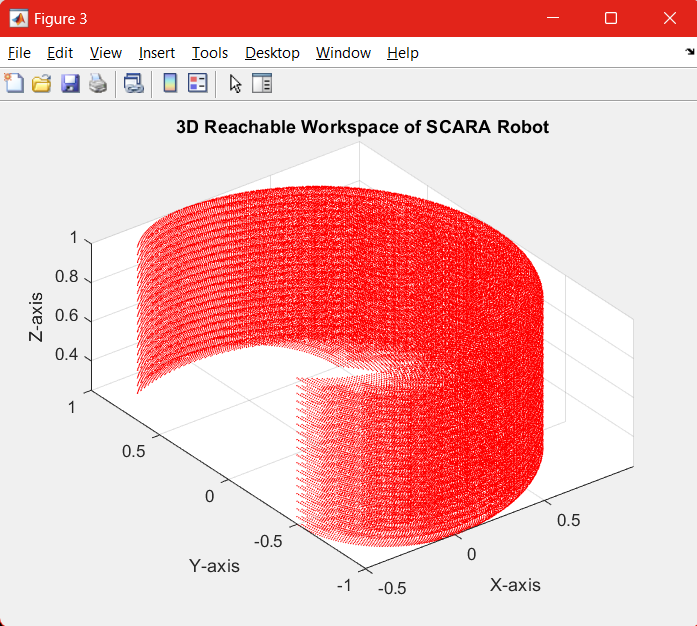
\includegraphics[scale=1]{W1} % Adjust the file path and scale as needed
	\caption{3D View of the Working Space}
	\label{W} % Add a label for referencing this figure
\end{figure}
\begin{figure}[H]
	\centering
	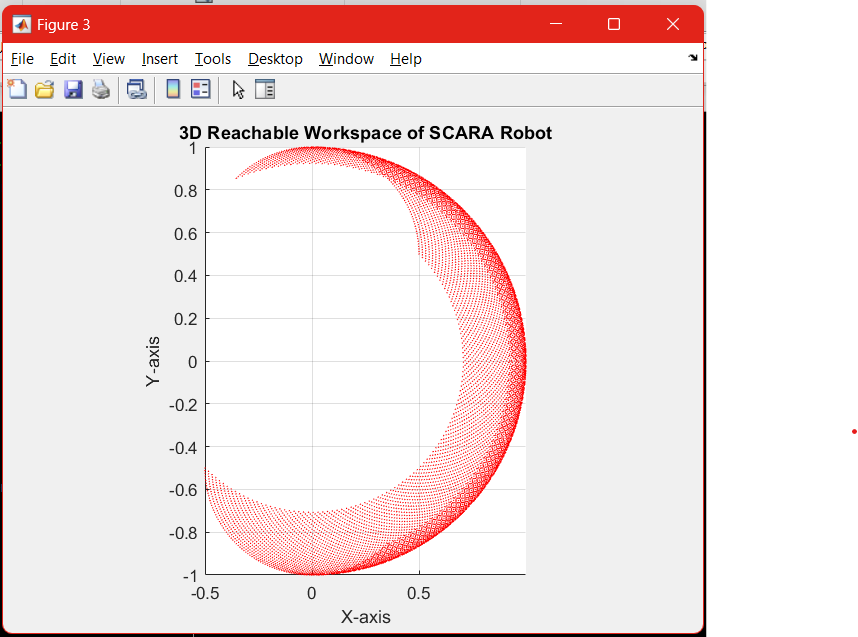
\includegraphics[scale=1]{W2} % Adjust the file path and scale as needed
	\caption{XY Plane View of the Working Space}
	\label{W2} % Add a label for referencing this figure
\end{figure}
\begin{figure}[H]
	\centering
	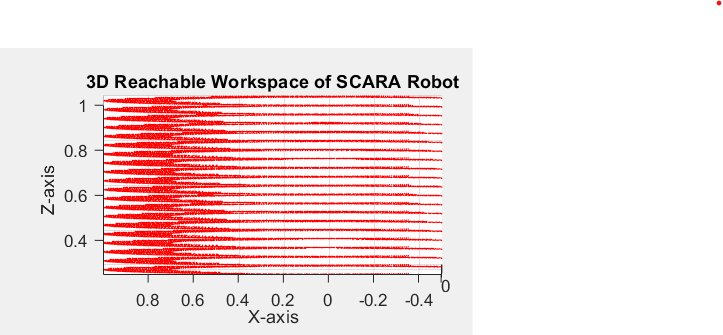
\includegraphics[scale=1]{W3} % Adjust the file path and scale as needed
	\caption{ZX Plane View of the Working Space}
	\label{W3} % Add a label for referencing this figure
\end{figure}

	\chapter{Jacobian}
		\addtocounter{section}{3} 
			\addtocounter{subsection}{0}
	\subsection{Geometric Jacobian}
	The Geometric Jacobian will be computed using the following procedure:
	
	\[
	\begin{bmatrix}
		\mathbf{J}_{\mathbf{P}_i} \\
		\mathbf{J}_{\mathbf{O}_i}
	\end{bmatrix}
	=
	\begin{cases} 
		\begin{bmatrix}
			\mathbf{z}_{i-1} \\
			\mathbf{0}
		\end{bmatrix}, & \text{for a \textit{prismatic} joint} \\
		\begin{bmatrix}
			\mathbf{z}_{i-1} \times (\mathbf{p} - \mathbf{p}_{i-1}) \\
			\mathbf{z}_{i-1}
		\end{bmatrix}, & \text{for a \textit{revolute} joint}
	\end{cases}
	\]\\
For our SCARA robot, the Jacobian will be in the form below.
\begin{equation}
	\mathbf{J}(\mathbf{q}) = \left[\begin{array}{cccc}
		\mathbf{Z}_0 \times\left(\mathbf{p} - \mathbf{p}_0\right) & \mathbf{Z}_1 \times\left(\mathbf{p} - \mathbf{p}_1\right) & \mathbf{Z}_2 & \mathbf{Z}_3 \times\left(\mathbf{p} - \mathbf{p}_3\right) \\
		\mathbf{Z}_0 & \mathbf{Z}_1 & 0 & \mathbf{Z}_3
	\end{array}\right]
\end{equation}\\
In order to solve the geometrical jacobian we have to recall the position of each joint which will require the homogenous transformation matrix calculated earlier on in Chapter 2, Section 1.1.1. The homogenous transformation matrix of each joint can be given as follows;\\
	\begin{equation}
		T_1^b=\left[\begin{array}{cccc}
			\cos \theta_1 & -\sin \theta_1 & 0 & 0 \\
			\sin \theta_1 & \cos \theta_1 & 0 & 0 \\
			0 & 0 & 1 & d_0 \\
			0 & 0 & 0 & 1
		\end{array}\right]
	\end{equation}
\begin{equation}
		T_1^b. T_2^1= 
	\begin{bmatrix}
		\cos(\theta_1 + \theta_2) & -\sin(\theta_1 + \theta_2) & 0 & -a_1 \cdot \sin(\theta_1) \\
		\sin(\theta_1 + \theta_2) & \cos(\theta_1 + \theta_2) & 0 & a_1 \cdot \cos(\theta_1) \\
		0 & 0 & 1 & d_o \\
		0 & 0 & 0 & 1
	\end{bmatrix}
\end{equation}
\begin{equation}
	T_1^b. T_2^1.T_3^1=
	\begin{bmatrix}
		\cos(\theta_1 + \theta_2) & -\sin(\theta_1 + \theta_2) & 0 & -a_1 \cdot \sin(\theta_1) - a_2 \cdot \sin(\theta_1 + \theta_2) \\
		\sin(\theta_1 + \theta_2) & \cos(\theta_1 + \theta_2) & 0 & a_1 \cdot \cos(\theta_1) + a_2 \cdot \cos(\theta_1 + \theta_2) \\
		0 & 0 & 1 & d_3 + d_o \\
		0 & 0 & 0 & 1
	\end{bmatrix}
\end{equation}

\begin{equation}
	T_1^b. T_2^1.T_3^2.T_e^3=
	\begin{bmatrix}
		\cos(\theta_1 + \theta_2 + \theta_4) & -\sin(\theta_1 + \theta_2 + \theta_4) & 0 & -a_1 \cdot \sin(\theta_1) - a_2 \cdot \sin(\theta_1 + \theta_2) \\
		\sin(\theta_1 + \theta_2 + \theta_4) & \cos(\theta_1 + \theta_2 + \theta_4) & 0 & a_1 \cdot \cos(\theta_1) + a_2 \cdot \cos(\theta_1 + \theta_2) \\
		0 & 0 & -1 & d_3 + d_o \\
		0 & 0 & 0 & 1
	\end{bmatrix}
\end{equation}
Where equation 3.1, 3.2, 3.3 and 3.4 resolves to the matrix at each joints. From here, we can get the $(P_i$) of each joint i.
From the above set of equations, it is easy to deduce that;
\begin{equation}
	\mathbf{Z}_0 = \mathbf{Z}_1 = \mathbf{Z}_2 = \mathbf{Z}_3 = 
	\begin{bmatrix}
		0 \\
		0 \\
		1
	\end{bmatrix}
\end{equation}
\begin{equation}
	\textbf{p} =
	\begin{bmatrix}
		-a_1 \cdot \sin(\theta_1) - a_2 \cdot \sin(\theta_1 + \theta_2) \\
		a_1 \cdot \cos(\theta_1) + a_2 \cdot \cos(\theta_1 + \theta_2) \\
		d_3 + d_o \\
		1
	\end{bmatrix}
\end{equation}
\begin{equation}
	\mathbf{P}_0 = 
	\begin{bmatrix}
		0 \\
		0 \\
		0
	\end{bmatrix}
\end{equation}


	\begin{equation}
	\textbf{p}_1=\left[\begin{array}{cccc}
		 0 \\
	 0 \\
	 d_0 \\
	 1
	\end{array}\right]
\end{equation}
\begin{equation}
	\textbf{p}_2= 
	\begin{bmatrix}
		 -a_1 \cdot \sin(\theta_1) \\
	 a_1 \cdot \cos(\theta_1) \\
	d_o \\
	1
	\end{bmatrix}
\end{equation}
\begin{equation}
	\textbf{p}_3=
	\begin{bmatrix}
		-a_1 \cdot \sin(\theta_1) - a_2 \cdot \sin(\theta_1 + \theta_2) \\
	 a_1 \cdot \cos(\theta_1) + a_2 \cdot \cos(\theta_1 + \theta_2) \\
	d_3 + d_o \\
1
	\end{bmatrix}
\end{equation}

Linear Velocity Component $\left(J_p\right)$ :

\begin{equation}
	J_p = \left[\begin{array}{llll}
		Z_0 \times\left(p-p_0\right) & Z_1 \times\left(p-p_1\right) & Z_2 & Z_3 \times\left(p-p_3\right)
	\end{array}\right]
\end{equation}

1. For $Z_0 \times\left(p-p_0\right)$ :

\begin{equation}
	p - p_0 = p_3 - p_0 =
	\begin{bmatrix}
		-a_1 \sin \theta_1 - a_2 \sin (\theta_1 + \theta_2) \\
		a_1 \cos \theta_1 + a_2 \cos (\theta_1 + \theta_2) \\
		d_3 + d_0
	\end{bmatrix}
\end{equation}

\begin{equation}
	Z_0 \times (p - p_0) =
	\begin{bmatrix}
		-\left(a_1 \cos \theta_1 + a_2 \cos (\theta_1 + \theta_2)\right) \\
		-\left(a_1 \sin \theta_1 + a_2 \sin (\theta_1 + \theta_2)\right) \\
		0
	\end{bmatrix}
\end{equation}


2. For $Z_1 \times\left(p-p_1\right)$ :

\begin{equation}
	p - p_1 = p_3 - p_1 =
	\begin{bmatrix}
		-a_1 \sin \theta_1 - a_2 \sin (\theta_1 + \theta_2) \\
		a_1 \cos \theta_1 + a_2 \cos (\theta_1 + \theta_2) \\
		d_3
	\end{bmatrix}
\end{equation}

\begin{equation}
	Z_1 \times (p - p_1) =
	\begin{bmatrix}
		-a_2 \cos (\theta_1 + \theta_2) \\
		-a_2 \sin (\theta_1 + \theta_2) \\
		0
	\end{bmatrix}
\end{equation}


3. For $Z_2$ :

\begin{equation}
	Z_2 =
	\begin{bmatrix}
		0 \\
		0 \\
		1
	\end{bmatrix}
\end{equation}


4. For $Z_3 \times\left(p-p_3\right)$ :

\begin{equation}
	p - p_3 =
	\begin{bmatrix}
		0 \\
		0 \\
		0
	\end{bmatrix}
\end{equation}

\begin{equation}
	Z_3 \times (p - p_3) =
	\begin{bmatrix}
		0 \\
		0 \\
		0
	\end{bmatrix}
\end{equation}

Angular Velocity Component $\left(J_o\right)$ :

\begin{equation}
	J_o = 
	\begin{bmatrix}
		Z_0 & Z_1 & 0 & Z_3
	\end{bmatrix}
\end{equation}

\begin{equation}
	J_o = 
	\begin{bmatrix}
		\begin{bmatrix}
			0 \\ 
			0 \\ 
			1
		\end{bmatrix}, 
		\begin{bmatrix}
			0 \\ 
			0 \\ 
			1
		\end{bmatrix}, 
		\begin{bmatrix}
			0 \\ 
			0 \\ 
			0
		\end{bmatrix}, 
		\begin{bmatrix}
			0 \\ 
			0 \\ 
			1
		\end{bmatrix}
	\end{bmatrix}
\end{equation}

Final Geometric Jacobian:

\begin{equation}
	J(q) =
	\begin{bmatrix}
		-\left(a_1 \cos \theta_1 + a_2 \cos (\theta_1 + \theta_2)\right) & -a_2 \cos (\theta_1 + \theta_2) & 0 & 0 \\
		-\left(a_1 \sin \theta_1 + a_2 \sin (\theta_1 + \theta_2)\right) & -a_2 \sin (\theta_1 + \theta_2) & 0 & 0 \\
		0 & 0 & 1 & 0 \\
		0 & 0 & 0 & 0 \\
		0 & 0 & 0 & 0 \\
		1 & 1 & 0 & 1
	\end{bmatrix}
\end{equation}


This Jacobian matrix $J(q)$ captures the relationship between the joint velocities $\dot{q}=$ $\left[\dot{\theta}_1, \dot{\theta}_2, \dot{d}_3, \dot{\theta}_4\right]^T$ and the end-effector velocities. 

\subsubsection{Verification with Corke's Robotics Toolbox}
\begin{figure}[H]
	\centering
	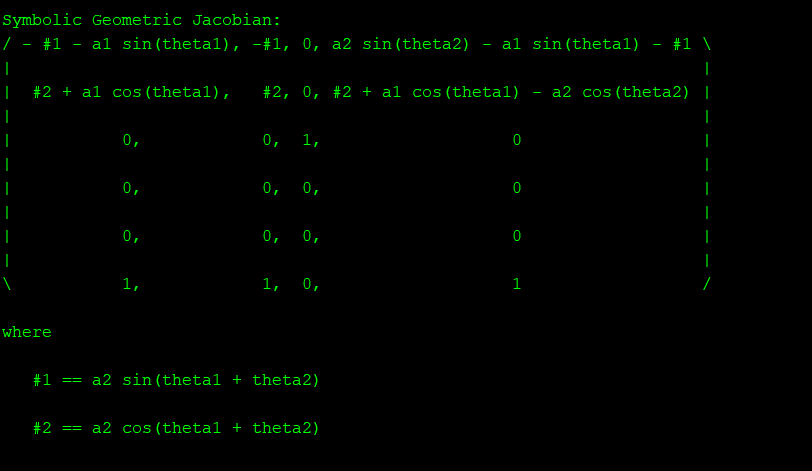
\includegraphics[scale=1]{run9} % Adjust the file path and scale as needed
	\caption{Verification of Geometric Jacobian from Corke's Robotics Toolbox}
	\label{run9} % Add a label for referencing this figure
\end{figure}





\subsubsection{Comparison and Proof}
The result from the Corke Robotics Toolbox for the fourth column is:
\[
\begin{bmatrix}
	a_2 \sin(\theta_2) - a_1 \sin(\theta_1) - \#1 \\
	a_2 \cos(\theta_2) + a_1 \cos(\theta_1) - \#2 \\
	0 \\
	0 \\
	0 \\
	1
\end{bmatrix}
\]
where:
- \(\#1 = a_2 \sin(\theta_1 + \theta_2)\),
- \(\#2 = a_2 \cos(\theta_1 + \theta_2)\).
\\1. Linear Velocity Contribution (\(J_p\)) for the Fourth Column:
- The Corke result indicates that \(\theta_4\) has additional contributions to the \(x\) and \(y\) directions due to the geometry of the robot:
\[
J_p(:,4) =
\begin{bmatrix}
	a_2 \sin(\theta_2) - a_1 \sin(\theta_1) - \#1 \\
	a_2 \cos(\theta_2) + a_1 \cos(\theta_1) - \#2 \\
	0
\end{bmatrix}
\]
- This makes sense geometrically: even though \(\theta_4\) primarily affects rotation about the Z-axis, its effect on the end-effector's orientation can also create small shifts in the \(x\) and \(y\)-directions due to the arm configuration.

2. Angular Velocity Contribution (\(J_o\)) for the Fourth Column:
- Both our derivation and Corke's result agree:
\[
J_o(:,4) =
\begin{bmatrix}
	0 \\ 0 \\ 1
\end{bmatrix}
\]

3. Agreement for Columns 1–3:
- Columns 1–3 of the Jacobian are identical in both the manual derivation and Corke's output. These terms are straightforward and follow from the forward kinematics.

4. Conclusion:
- The Corke Robotics Toolbox incorporates additional effects of \(\theta_4\) on the linear velocities, which were neglected in the manual derivation. These contributions depend on the robot's configuration and become more apparent when higher-order effects (small displacements due to \(\theta_4\)) are considered.

The Jacobian from Corke Robotics Toolbox is more comprehensive and accurate because it accounts for these subtle effects. Therefore:
The Toolbox result is correct and more complete.
The manual derivation is an approximation and assumes \(\theta_4\) affects only the angular velocity.

\subsection{Analytical Jacobian}
The analytical Jacobian relates the joint velocities $\dot{q}=\left[\dot{\theta}_1, \dot{\theta}_2, \dot{d}_3, \dot{\theta}_4\right]$ to the linear velocity $(\dot{p})$ and angular velocity $(\omega)$ of the end-effector. It is derived using the position equations from forward kinematics.

Forward Kinematics of the SCARA Robot
The position of the end-effector is given by:

\begin{equation}
	x = a_1 \cos \left(\theta_1\right) + a_2 \cos \left(\theta_1 + \theta_2\right)
\end{equation}

\begin{equation}
	y = a_1 \sin \left(\theta_1\right) + a_2 \sin \left(\theta_1 + \theta_2\right)
\end{equation}

\begin{equation}
	z = d_0 + d_3
\end{equation}


The orientation of the end-effector is described by $\theta_4$, the rotation angle about the Z -axis.
1. Partial Derivatives for Linear Velocity $\left(J_p\right)$ :

The linear velocity $\dot{p}=[\dot{x}, \dot{y}, \dot{z}]$ is derived by taking partial derivatives of $x, y$, and $z$ with respect to the joint variables $\theta_1, \theta_2, d_3$, and $\theta_4$.
\\For $x$ :

\begin{equation}
	\frac{\partial x}{\partial \theta_1} = -a_1 \sin \left(\theta_1\right) - a_2 \sin \left(\theta_1 + \theta_2\right)
\end{equation}

\begin{equation}
	\frac{\partial x}{\partial \theta_2} = -a_2 \sin \left(\theta_1 + \theta_2\right)
\end{equation}

\begin{equation}
	\frac{\partial x}{\partial d_3} = 0
\end{equation}

\begin{equation}
	\frac{\partial x}{\partial \theta_4} = 0
\end{equation}

For $y$ :

\begin{equation}
	\frac{\partial y}{\partial \theta_1} = a_1 \cos \left(\theta_1\right) + a_2 \cos \left(\theta_1 + \theta_2\right)
\end{equation}

\begin{equation}
	\frac{\partial y}{\partial \theta_2} = a_2 \cos \left(\theta_1 + \theta_2\right)
\end{equation}

\begin{equation}
	\frac{\partial y}{\partial d_3} = 0
\end{equation}

\begin{equation}
	\frac{\partial y}{\partial \theta_4} = 0
\end{equation}


For z:

\begin{equation}
	\frac{\partial z}{\partial \theta_1} = 0
\end{equation}

\begin{equation}
	\frac{\partial z}{\partial \theta_2} = 0
\end{equation}

\begin{equation}
	\frac{\partial z}{\partial d_3} = 1
\end{equation}

\begin{equation}
	\frac{\partial z}{\partial \theta_4} = 0
\end{equation}


2. Partial Derivatives for Angular Velocity $\left(J_o\right)$ :

The angular velocity is influenced only by the rotational joints $\left(\theta_1, \theta_2, \theta_4\right)$. Since all rotations are about the Z-axis:

\begin{equation}
	\omega = 
	\begin{bmatrix}
		0 \\
		0 \\
		\dot{\theta}_1 + \dot{\theta}_2 + \dot{\theta}_4
	\end{bmatrix}
\end{equation}



Therefore:

\begin{equation}
	J_o =
	\begin{bmatrix}
		0 & 0 & 0 & 0 \\
		0 & 0 & 0 & 0 \\
		1 & 1 & 0 & 1
	\end{bmatrix}
\end{equation}

3. Combine $J_p$ and $J_o$ :

Using the partial derivatives calculated above, we construct the full analytical Jacobian:

\begin{equation}
	J =
	\begin{bmatrix}
		\frac{\partial x}{\partial \theta_1} & \frac{\partial x}{\partial \theta_2} & \frac{\partial x}{\partial d_3} & \frac{\partial x}{\partial \theta_4} \\
		\frac{\partial y}{\partial \theta_1} & \frac{\partial y}{\partial \theta_2} & \frac{\partial y}{\partial d_3} & \frac{\partial y}{\partial \theta_4} \\
		\frac{\partial z}{\partial \theta_1} & \frac{\partial z}{\partial \theta_2} & \frac{\partial z}{\partial d_3} & \frac{\partial z}{\partial \theta_4} \\
		0 & 0 & 0 & 0 \\
		0 & 0 & 0 & 0 \\
		1 & 1 & 0 & 1
	\end{bmatrix}
\end{equation}



Substituting the partial derivatives:

\begin{equation}
	J =
	\begin{bmatrix}
		\frac{\partial x}{\partial \theta_1} & \frac{\partial x}{\partial \theta_2} & \frac{\partial x}{\partial d_3} & \frac{\partial x}{\partial \theta_4} \\
		\frac{\partial y}{\partial \theta_1} & \frac{\partial y}{\partial \theta_2} & \frac{\partial y}{\partial d_3} & \frac{\partial y}{\partial \theta_4} \\
		\frac{\partial z}{\partial \theta_1} & \frac{\partial z}{\partial \theta_2} & \frac{\partial z}{\partial d_3} & \frac{\partial z}{\partial \theta_4} \\
		0 & 0 & 0 & 0 \\
		0 & 0 & 0 & 0 \\
		1 & 1 & 0 & 1
	\end{bmatrix}
\end{equation}

1. Angular Velocity in Terms of Euler Angles

For a SCARA robot, if the orientation of the end-effector is represented using ZYZ Euler angles ( $\phi, \theta, \psi)$, the angular velocity $\omega=\left[\omega_x, \omega_y, \omega_z\right]^T$ can be related to the time derivatives of the Euler angles $[\dot{\phi}, \dot{\theta}, \dot{\psi}]$ via a transformation matrix $T_E$ :

\begin{equation}
	\omega = T_E
	\begin{bmatrix}
		\dot{\phi} \\
		\dot{\theta} \\
		\dot{\psi}
	\end{bmatrix}
\end{equation}


The transformation matrix $T_E$ for ZYZ Euler angles is:

\begin{equation}
	T_E =
	\begin{bmatrix}
		0 & -\sin (\phi) & \cos (\phi) \sin (\theta) \\
		0 & \cos (\phi) & \sin (\phi) \sin (\theta) \\
		1 & 0 & \cos (\theta)
	\end{bmatrix}
\end{equation}

2. Compute the Analytical Jacobian with Euler Angles

The analytical Jacobian relates the joint velocities $\left(\dot{q}=\left[\dot{\theta}_1, \dot{\theta}_2, \dot{d}_3, \dot{\theta}_4\right]^T\right)$ to:
1. The linear velocity $(\dot{p})$.
2. The time derivatives of the Euler angles $([\dot{\phi}, \dot{\theta}, \dot{\psi}])$.

The analytical Jacobian $J_A$ is computed as:

\begin{equation}
	\begin{bmatrix}
		\dot{p} \\
		\begin{bmatrix}
			\dot{\phi} \\
			\dot{\theta} \\
			\dot{\psi}
		\end{bmatrix}
	\end{bmatrix}
	=
	\begin{bmatrix}
		J_p \\
		T_E^{-1} J_o
	\end{bmatrix} \dot{q}
\end{equation}


Here:
\\$J_p$ : Linear velocity Jacobian (from forward kinematics).
\\$J_o$ : Angular velocity Jacobian (relating joint velocities to $\omega$ ).
\\$T_E^{-1}$ : Inverse of the transformation matrix that maps $\omega$ to the time derivatives of the Euler angles.
\\\\3. Steps to Compute the Analytical Jacobian

Step 1: Linear Velocity Jacobian ( $J_p$ )
From forward kinematics:

\begin{equation}
	J_p =
	\begin{bmatrix}
		-\left(a_1 \sin \left(\theta_1\right) + a_2 \sin \left(\theta_1 + \theta_2\right)\right) & -a_2 \sin \left(\theta_1 + \theta_2\right) & 0 & 0 \\
		a_1 \cos \left(\theta_1\right) + a_2 \cos \left(\theta_1 + \theta_2\right) & a_2 \cos \left(\theta_1 + \theta_2\right) & 0 & 0 \\
		0 & 0 & 1 & 0
	\end{bmatrix}
\end{equation}



Step 2: Angular Velocity Jacobian ( $J_o$ )
The angular velocity Jacobian is:

\begin{equation}
	J_o =
	\begin{bmatrix}
		0 & 0 & 0 & 0 \\
		0 & 0 & 0 & 0 \\
		1 & 1 & 0 & 1
	\end{bmatrix}
\end{equation}



Step 3: Inverse of Transformation Matrix ( $T_E^{-1}$ )
The inverse of $T_E$ is given by:

\begin{equation}
	T_E^{-1} =
	\begin{bmatrix}
		0 & 0 & 1 \\
		-\sin (\phi) & \cos (\phi) & 0 \\
		\cos (\phi) \sin (\theta) & \sin (\phi) \sin (\theta) & \cos (\theta)
	\end{bmatrix}
\end{equation}



Step 4: Combine Linear and Angular Components
To compute the full analytical Jacobian:

\begin{equation}
	J_A =
	\begin{bmatrix}
		J_p \\
		T_E^{-1} J_o
	\end{bmatrix}
\end{equation}

4. Final Analytical Jacobian

Substituting $J_{p,} J_o$, and $T_E^{-1}$, the final analytical Jacobian becomes:

\begin{equation}
	J_A =
	\begin{bmatrix}
		-\left(a_1 \sin \left(\theta_1\right) + a_2 \sin \left(\theta_1 + \theta_2\right)\right) & -a_2 \sin \left(\theta_1 + \theta_2\right) & 0 & 0 \\
		a_1 \cos \left(\theta_1\right) + a_2 \cos \left(\theta_1 + \theta_2\right) & a_2 \cos \left(\theta_1 + \theta_2\right) & 0 & 0 \\
		0 & 0 & 1 & 0 \\
		0 & 0 & 1 & 0 \\
		-\sin (\phi) & \cos (\phi) & 0 & 0 \\
		\cos (\phi) \sin (\theta) & \sin (\phi) \sin (\theta) & \cos (\theta) & 0
	\end{bmatrix}
\end{equation}



This Jacobian now relates $\dot{q}$ to the linear velocity $(\dot{p})$ and Euler angle rates $([\dot{\phi}, \dot{\theta}, \dot{\psi}]$ ).

\subsubsection*{Key Considerations}
1. The other Euler angles such as $\theta=0^{\circ}$ because of the nature of our end-effector.
\\\\So the matrix becomes:\\
\begin{equation}
	J_A =
	\begin{bmatrix}
		-\left(a_1 \sin \left(\theta_1\right) + a_2 \sin \left(\theta_1 + \theta_2\right)\right) & -a_2 \sin \left(\theta_1 + \theta_2\right) & 0 & 0 \\
		a_1 \cos \left(\theta_1\right) + a_2 \cos \left(\theta_1 + \theta_2\right) & a_2 \cos \left(\theta_1 + \theta_2\right) & 0 & 0 \\
		0 & 0 & 1 & 0 \\
		0 & 0 & 1 & 0 \\
		-\sin (\phi) & \cos (\phi) & 0 & 0 \\
		0 & 0 & 1 & 0
	\end{bmatrix}
\end{equation}

\subsubsection{Verification with Corke's Robotics Toolbox}
\begin{figure}[H]
	\centering
	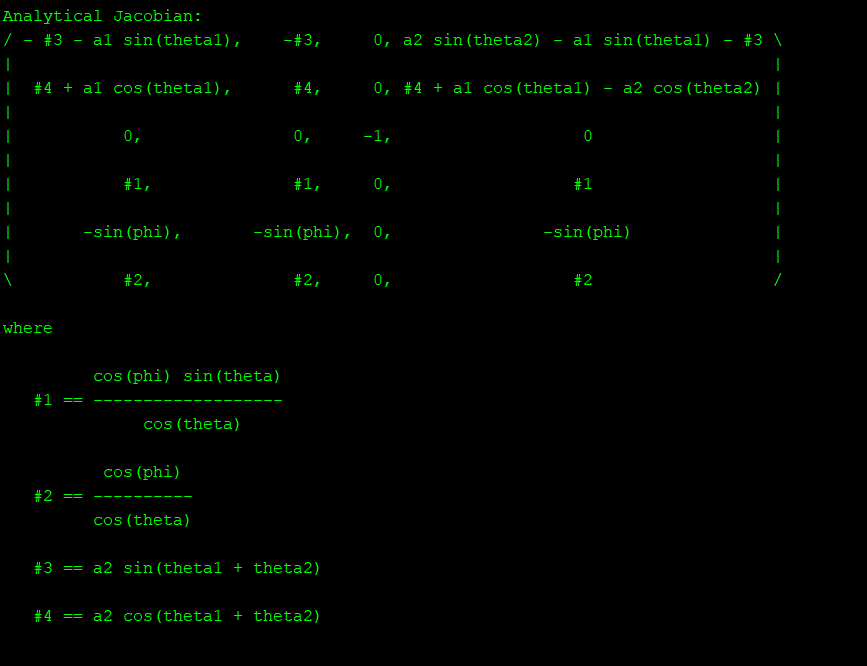
\includegraphics[scale=1]{run10} % Adjust the file path and scale as needed
	\caption{Verification of Analytical Jacobian from Corke's Robotics Toolbox}
	\label{run10} % Add a label for referencing this figure
\end{figure}
	\chapter{Trajectory Planning}
		\addtocounter{section}{4} 
	\addtocounter{subsection}{0}
	The workspace of a robotic manipulator represents the region in 3D space that the end-effector can reach, based on its kinematic configuration, joint limits, and link lengths. In this chapter, I go into the details and the methods used to determine the workspace mathematically and computationally. I also describe how linear and circular trajectories within the workspace were mathematically defined and implemented in MATLAB.
	
	\subsection{Mathematical Derivation for Linear and Circular Paths}
	
	\subsubsection{Linear Trajectory}
	
	The linear trajectory is computed to interpolate between two points \( \mathbf{P}_{\text{start}} \) and \( \mathbf{P}_{\text{end}} \) in 3D space over a defined time interval \([t_{\text{start}}, t_{\text{end}}]\). The formula for this trajectory is derived as follows:
	
	1. Normalized Time Parameter (\(\tau\)):
	The time \(t\) is normalized to a parameter \(\tau \in [0, 1]\), which represents the progression along the path:
\begin{equation}
	\tau = \frac{t - t_{\text{start}}}{t_{\text{end}} - t_{\text{start}}}
\end{equation}

	Here:
	\(\tau = 0\) corresponds to \(t = t_{\text{start}}\),
	 \(\tau = 1\) corresponds to \(t = t_{\text{end}}\).
	
	2. Linear Interpolation:
	The interpolated position \(\mathbf{P}(t)\) is a weighted combination of the start and end points:
	\begin{equation}
		\mathbf{P}(t) = (1 - \tau) \mathbf{P}_{\text{start}} + \tau \mathbf{P}_{\text{end}}
	\end{equation}
	
	Expanding this:
	\begin{equation}
		\mathbf{P}(t) = \mathbf{P}_{\text{start}} + \tau (\mathbf{P}_{\text{end}} - \mathbf{P}_{\text{start}})
	\end{equation}
	
	This formula provides a smooth linear transition between the two points.
	
	3. Algorithm in the Matlab Code:
	- For \(n\) time steps, the function iterates over \(t\), calculates \(\tau\) for each step, and computes the corresponding point:
	
	\begin{center}
		\textbf{\texttt{tau = (t(i) - t\_start) / (t\_end - t\_start); \\
				segment(i, :) = P\_start + tau * (P\_end - P\_start);}}
	\end{center}
	
	
	\subsubsection{Circular Trajectory}
	
	The circular trajectory is computed to interpolate between two points \( \mathbf{P}_{\text{start}} \) and \( \mathbf{P}_{\text{end}} \) lying on a circular arc. The trajectory is defined by the center and radius of the circle and the angular span between the two points.
	
	1. Defining the Circle:
	The radius of the circle is given by:
\begin{equation}
	\text{radius} = \frac{\|\mathbf{P}_{\text{end}} - \mathbf{P}_{\text{start}}\|}{2}
\end{equation}

	The center of the circle lies midway between the two points:
\begin{equation}
	\text{center} = \frac{\mathbf{P}_{\text{start}} + \mathbf{P}_{\text{end}}}{2}
\end{equation}

	
	2. Angles of the Arc:
	The angular positions of \(\mathbf{P}_{\text{start}}\) and \(\mathbf{P}_{\text{end}}\) relative to the center are calculated using the \(\text{atan2}\) function:
\begin{equation}
	\theta_{\text{start}} = \tan^{-1} \left( \frac{P_{\text{start},y} - \text{center}_y}{P_{\text{start},x} - \text{center}_x} \right)
\end{equation}
\begin{equation}
	\theta_{\text{end}} = \tan^{-1} \left( \frac{P_{\text{end},y} - \text{center}_y}{P_{\text{end},x} - \text{center}_x} \right)
\end{equation}

	3. Parametric Representation:
	The circular arc is parametrized by an angle \(\theta(t)\), which is interpolated linearly between \(\theta_{\text{start}}\) and \(\theta_{\text{end}}\):
\begin{equation}
	\theta(t) = \theta_{\text{start}} + \tau (\theta_{\text{end}} - \theta_{\text{start}})
\end{equation}

	The corresponding position in the \(x\)-\(y\) plane is:
\begin{equation}
	P_x(t) = \text{center}_x + \text{radius} \cdot \cos(\theta(t))
\end{equation}
\begin{equation}
	P_y(t) = \text{center}_y + \text{radius} \cdot \sin(\theta(t))
\end{equation}

	4. Linear Interpolation for \(z\):
	Since the \(z\)-component is not affected by the circular motion, it is interpolated linearly:
\begin{equation}
	P_z(t) = P_{\text{start},z} + \tau (P_{\text{end},z} - P_{\text{start},z})
\end{equation}

	
	5. Algorithm in the Matlab Code:
	The function computes the normalized time \(\tau\) and interpolates the angle \(\theta(t)\) for each time step:
	
\begin{center}
	\textbf{\texttt{tau = (t(i) - t\_start) / (t\_end - t\_start); \\
			theta = theta\_start + tau * (theta\_end - theta\_start);}}
\end{center}

	
	The \(x\)-\(y\) positions are calculated using the cosine and sine of \(\theta\), and the \(z\)-position is interpolated linearly:
	
	\begin{center}
		\textbf{\texttt{
				segment(i, 1) = center(1) + radius * cos(theta); \\
				segment(i, 2) = center(2) + radius * sin(theta); \\
				segment(i, 3) = P\_start(3) + tau * (P\_end(3) - P\_start(3));}}
	\end{center}
	\subsubsection{Matlab Code}
	The following MATLAB code illustrates the computation of the robot's trajectory and workspace:
	

	
	\subsubsection{Result}
	
	\begin{figure}[H]
		\centering
		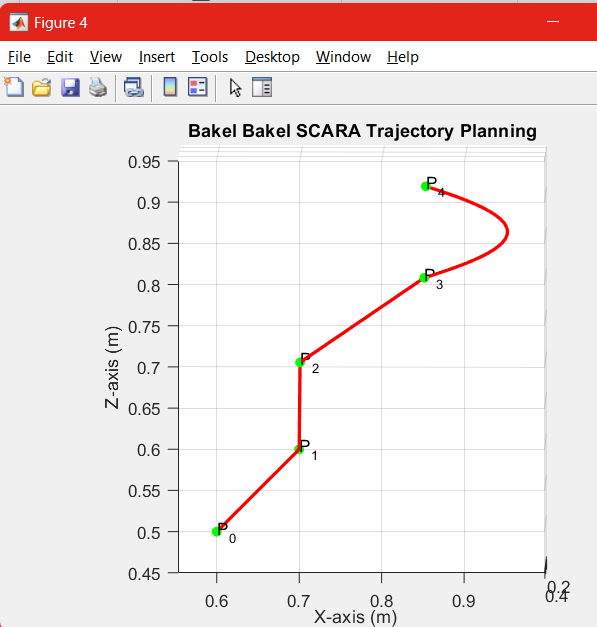
\includegraphics[scale=0.8]{T1} % Adjust the file path and scale as needed
		\caption{XZ Plane of the path}
		\label{run10} % Add a label for referencing this figure
	\end{figure}
	\begin{figure}[H]
		\centering
		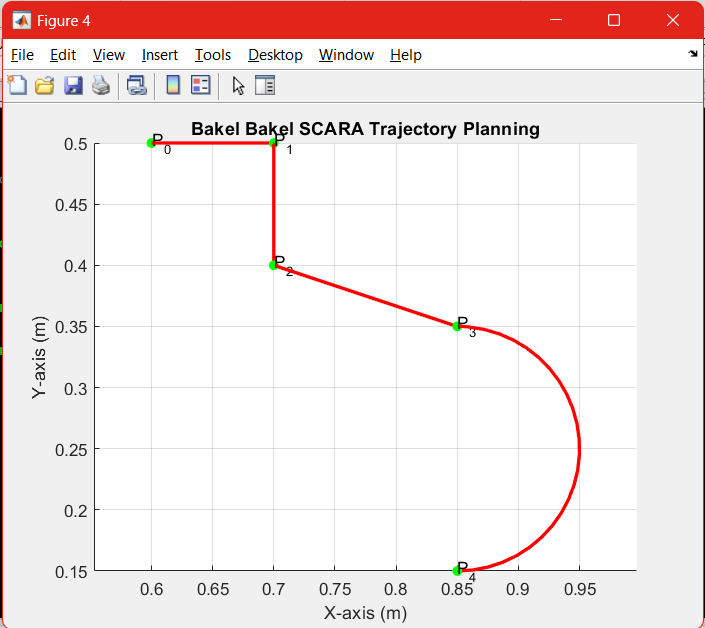
\includegraphics[scale=0.8]{T2} % Adjust the file path and scale as needed
		\caption{XY Plane of the path showing vertical and horizontal lines and circular section}
		\label{run10} % Add a label for referencing this figure
	\end{figure}
	\begin{figure}[H]
		\centering
		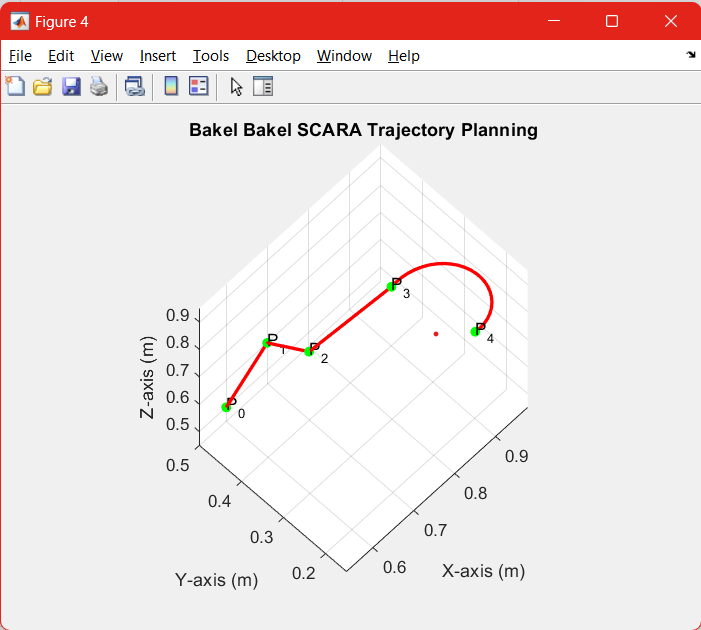
\includegraphics[scale=0.8]{T3} % Adjust the file path and scale as needed
		\caption{3D View of the planned path}
		\label{run10} % Add a label for referencing this figure
	\end{figure}
		\begin{figure}[H]
		\centering
		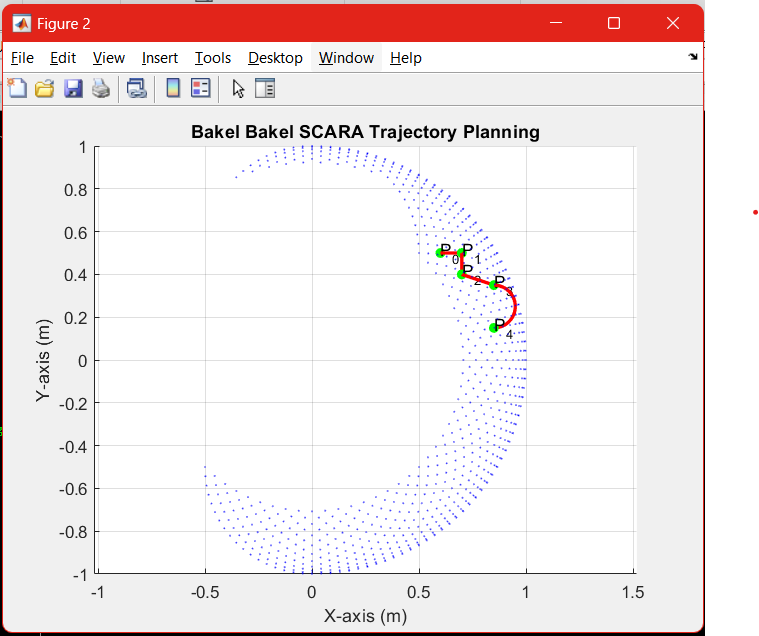
\includegraphics[scale=0.8]{PW1} % Adjust the file path and scale as needed
		\caption{XY Plane of the planned path and working space}
		\label{run10} % Add a label for referencing this figure
	\end{figure}
		\begin{figure}[H]
		\centering
		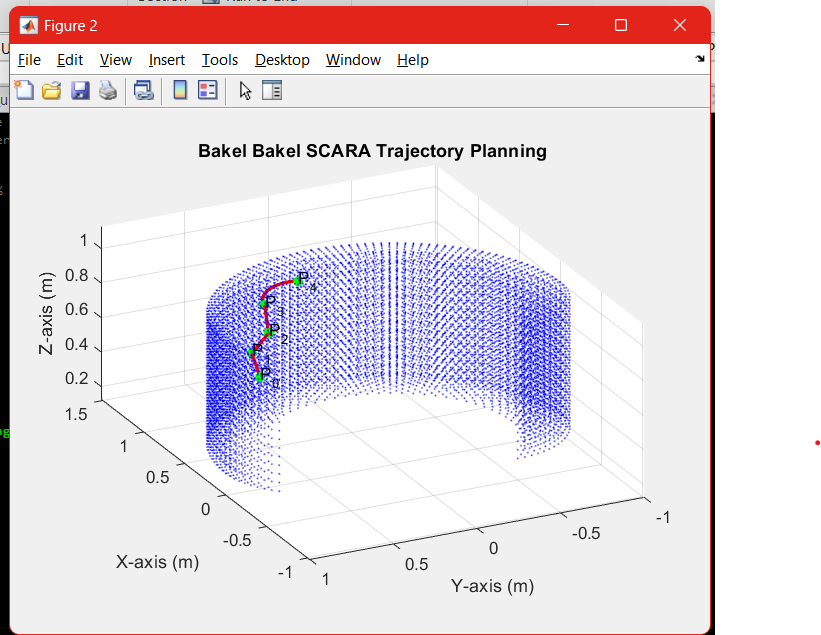
\includegraphics[scale=0.8]{PW2} % Adjust the file path and scale as needed
		\caption{3D View of the planned path and working space}
		\label{run10} % Add a label for referencing this figure
	\end{figure}
		\chapter{Kinematic Inversion with Inverse and Transpose of the Jacobian}
		
		
		In response to the number 5 question, 
		
		
		\begin{center}
			\textit{Implement in MATLAB or similar tool the algorithms for kinematic inversion with inverse and transpose of the Jacobian along the planned trajectory (adopt the Euler integration rule with an integration time of 1ms).}
		\end{center}
		I opted to directly code the solution in MATLAB. While Simulink offers a graphical approach to modeling and simulation, I chose MATLAB’s scripting environment for algorithm development because of its flexibility, precision, and finally I am more comfortable with the coding interface. However, for completeness and as a safety measure, I incorporated a Simulink model to provide an alternative visualization and validation of the results.
		\\\\The methodology involved using the inverse Jacobian and transpose Jacobian approaches to solve the kinematic inversion problem for a SCARA robot. These approaches were implemented along a planned trajectory (Chapter 4) in 3D operational space, ensuring the robot's end-effector accurately followed a predefined path. To integrate the algorithm over time, I adopted the Euler integration rule with a small time step of \(1 \, \text{ms}\), ensuring smooth transitions and accurate trajectory tracking.\\\\
		The fundamental concept behind the code lies in the Jacobian matrix, which maps joint velocities to end-effector velocities in operational space. \\For kinematic inversion:\\\\
		1. The inverse Jacobian method calculates joint velocities q that minimize the error between the desired and actual end-effector positions.\\
		2. The transpose Jacobian method calculates joint velocities by projecting the operational space error onto the rows of the transpose Jacobian, effectively using gradient descent to reduce the error.\\
		
		The planned trajectory was defined using waypoints that included both linear and circular segments. The operational space error (\(e\)) was computed at each time step as the difference between the desired and actual end-effector positions. The joint velocities were updated iteratively using the chosen kinematic inversion method and integrated over time using Euler's method to calculate the joint angles. These joint angles then drove the robot's motion along the planned trajectory.
		
		The implementation provided an opportunity to explore both theoretical and practical aspects of kinematic inversion. By opting for a direct MATLAB implementation, I was able to maintain low level control over the computations.
	
			\addtocounter{section}{5} 
		\addtocounter{subsection}{0}
		\subsection{Conceptual Background}
The Jacobian matrix, \(\mathbf{J} \in \mathbb{R}^{m \times n}\), represents the linear mapping between the joint space velocities, \(\dot{\mathbf{q}} \in \mathbb{R}^n\), and the end-effector velocities in the operational space, \(\dot{\mathbf{x}} \in \mathbb{R}^m\):

\[
\dot{\mathbf{x}} = \mathbf{J} \dot{\mathbf{q}}.
\]

For kinematic inversion, the goal is to compute the joint velocities, \(\dot{\mathbf{q}}\), that minimize the error, \(\mathbf{e} \in \mathbb{R}^m\), between the desired and current positions of the end-effector:

\[
\mathbf{e} = \mathbf{x}_{\text{desired}} - \mathbf{x}_{\text{current}}.
\]

	
		\subsubsection{Method 1: Inverse Jacobian}
		
		The inverse Jacobian method uses the Moore-Penrose pseudo-inverse of \(\mathbf{J}\) to compute the joint velocities:
	\[
	\dot{\mathbf{q}} = \mathbf{J}^\dagger \mathbf{e}.
	\]
	
		
		where,
		
		\[
		\mathbf{J}^\dagger = \mathbf{J}^T (\mathbf{J} \mathbf{J}^T)^{-1}, \quad \text{for } \mathbf{J} \in \mathbb{R}^{m \times n} \text{ and } m \leq n.
		\]
		
		This method ensures a least-squares solution, minimizing the norm of the error in operational space. It is particularly effective when the system is redundant or when the Jacobian is not square.
		
		\subsubsection{Method 2: Transpose Jacobian}
		
		The transpose Jacobian method computes the joint velocities by projecting the operational space error onto the rows of \(\mathbf{J}\):
\begin{equation}
	\dot{\mathbf{q}} = \mathbf{J}^T \mathbf{e}.
\end{equation}

		This approach can be interpreted as a gradient descent method, where the end-effector moves along the direction of maximum decrease in the error. While less computationally expensive than the inverse Jacobian method, it may converge more slowly.
		
		\subsection{Trajectory Planning and Execution}
		
		The trajectory was planned in operational space using waypoints, including both linear and circular segments. At each time step:\\\\
		1. The desired position of the end-effector, \(\mathbf{x_\text{desired}}(t)\), was determined based on the planned trajectory.\\
		2. The error, \(\mathbf{e}\), was computed between \(\mathbf{x_\text{desired}}(t)\) and the actual position, \(\mathbf{x_\text{current}}(t)\), obtained via forward kinematics.\\
		3. The joint velocities,\(\dot{\mathbf{q}}\), were calculated using the chosen kinematic inversion method (inverse or transpose Jacobian).\\
		4. The joint variables, \(\mathbf{q}(t)\), were updated using Euler's integration rule:\\
		\begin{equation}
			\mathbf{q}(t + \Delta t) = \mathbf{q}(t) + \Delta t \, \dot{\mathbf{q}}(t).
		\end{equation}
		
		
	
		\subsubsection{Explanation of the Pathway and Euler Angle \(\phi\)}
		
		In the planned trajectory for the SCARA robot, the path was defined exclusively in terms of the end-effector's position coordinates (\(x\), \(y\), and \(z\)) in operational space. The rotation of the end-effector, represented by the Euler angle \(\phi\), was not incorporated into the pathway definition. This means that while the robot follows the predefined path in 3D Cartesian space, the rotational degree of freedom (\(\phi\)) remains undefined and does not vary as the end-effector moves along the trajectory.\\The complete operational space for the robot end-effector typically includes both position (\(x, y, z\)) and orientation (\(\phi, \theta, \psi\), where \(\phi\) is the roll, \(\theta\) is the pitch, and \(\psi\) is the yaw).
		
		
		\subsubsection{Consequences of Not Defining \(\phi\)}
		
		1. Relaxation of Operational Space:\\By not explicitly defining \(\phi\), we implicitly allow the end-effector's rotation to vary freely. This relaxes the constraints in the operational space, leading to reduced control over the robot's behavior in the rotational dimension.
		
		2. Potential Inconsistencies:\\If the application requires the end-effector to maintain a specific orientation while moving along the trajectory (e.g., to grip or align with objects), not defining \(\phi\) could result in unintended rotations, causing task failures.
		
		3. Inefficient Use of Robot Degrees of Freedom (DoF):\\For a 4-DoF SCARA robot, failing to utilize \(\phi\) means only 3 of the 4 DoFs are actively contributing to the trajectory. This underutilizes the robot's capabilities and limits its functionality.
		
		
		\subsubsection{Explanation of Including \(q_4\) (\(\phi\)) in the Operational Space
		}
		To incorporate \(\phi\) into the pathway:\\\\
		1. Define \(\phi(t)\):
		Manually specify a variation for \(\phi\) as the robot moves along the trajectory. For example:
	\begin{equation}
		\phi(t) = \phi_0 + \omega t,
	\end{equation}
	
		where \(\phi_0\) is the initial angle, and \(\omega\) is the angular velocity.\\2. Modify the Error Vector: Include \(\phi\) in the error calculation:
	\begin{equation}
		\mathbf{e} = \mathbf{x}_{\text{desired}} - \mathbf{x}_{\text{current}},
	\end{equation}
	
		where:
		\begin{equation}
			\mathbf{x}_{\text{desired}} = [x_{\text{desired}}, y_{\text{desired}}, z_{\text{desired}}, \phi_{\text{desired}}]^T.
		\end{equation}
		3. Update the Jacobian Matrix:\\Retain the rotational component of the Jacobian (\(\mathbf{J}_{:,4}\)) to calculate the effect of \(\phi\) on joint velocities. 4. Logic Behind the Code To include \(\phi\) in the operational space, we introduced a predefined variation for \(q_4\) as the robot moved along the \(x, y, z\) trajectory. The logic was implemented as follows:
		
		The joint velocity for \(q_4\) was explicitly set to a constant rate (\(\omega\)) in the loop:
	\begin{figure}[H]
		\centering
		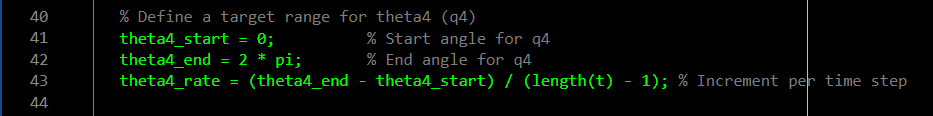
\includegraphics[scale=0.8]{Q1} % Adjust the file path and scale as needed
		\caption{Inclusion of Euler Angle to the Operational Space}
		\label{run10} % Add a label for referencing this figure
	\end{figure}
	3. Integration with the Full Operational Space:\\The error vector (\(\mathbf{e}\)) was extended to include \(\phi\), ensuring the Jacobian accounted for the rotational component:
	\begin{equation}
		\mathbf{e} = \begin{bmatrix}
			x_{\text{desired}} - x_{\text{current}} \\
			y_{\text{desired}} - y_{\text{current}} \\
			z_{\text{desired}} - z_{\text{current}} \\
			\phi_{\text{desired}} - \phi_{\text{current}}
		\end{bmatrix}.
	\end{equation}
	4. Updated Operational Space:\\The operational space was expanded to:
		\[
		\mathbf{x} = [x, y, z, \phi]^T,
		\]
		and the Jacobian matrix included the fourth column for \(\phi\).\\The full operational space velocity equation is:
	\[
	\dot{\mathbf{x}} = \mathbf{J} \dot{\mathbf{q}},
	\]
	
		where:
		\[
		\mathbf{J} =
		\begin{bmatrix}
			\mathbf{J}_{\text{pos}} \\
			\mathbf{J}_{\text{rot}}
		\end{bmatrix}.
		\]Initially, \(\mathbf{J}_{\text{rot}}\) (the rotational part) was ignored. By defining \(\phi\) and including it in the trajectory:\\\\
		1. The fourth row of the Jacobian was restored to account for rotational velocity.\\
		2. The pseudo-inverse of the Jacobian, \(\mathbf{J}^\dagger\), calculated joint velocities considering both positional (\(x, y, z\)) and rotational (\(\phi\)) errors:
		\[
		\dot{\mathbf{q}} = \mathbf{J}^\dagger \mathbf{e}.
		\]
		
		\subsubsection{Advantages of Defining \(\phi\)}1. Complete Utilization of the Operational Space:
		- Incorporating \(\phi\) ensured that all four degrees of freedom (\(q_1, q_2, q_3, q_4\)) contributed to the trajectory, maximizing the robot’s functionality.\\2. Precise Control of Orientation:
		- The robot was able to maintain or vary its orientation (\(\phi\)) as required for specific tasks, such as aligning with objects or performing rotational motions.\\3. Task Reliability:
		- For tasks involving manipulation, defining \(\phi\) ensures the end-effector maintains the correct orientation, improving reliability and efficiency.
		
		\subsection{Inverse Jacobian}
			\subsubsection{Code Implementation}
		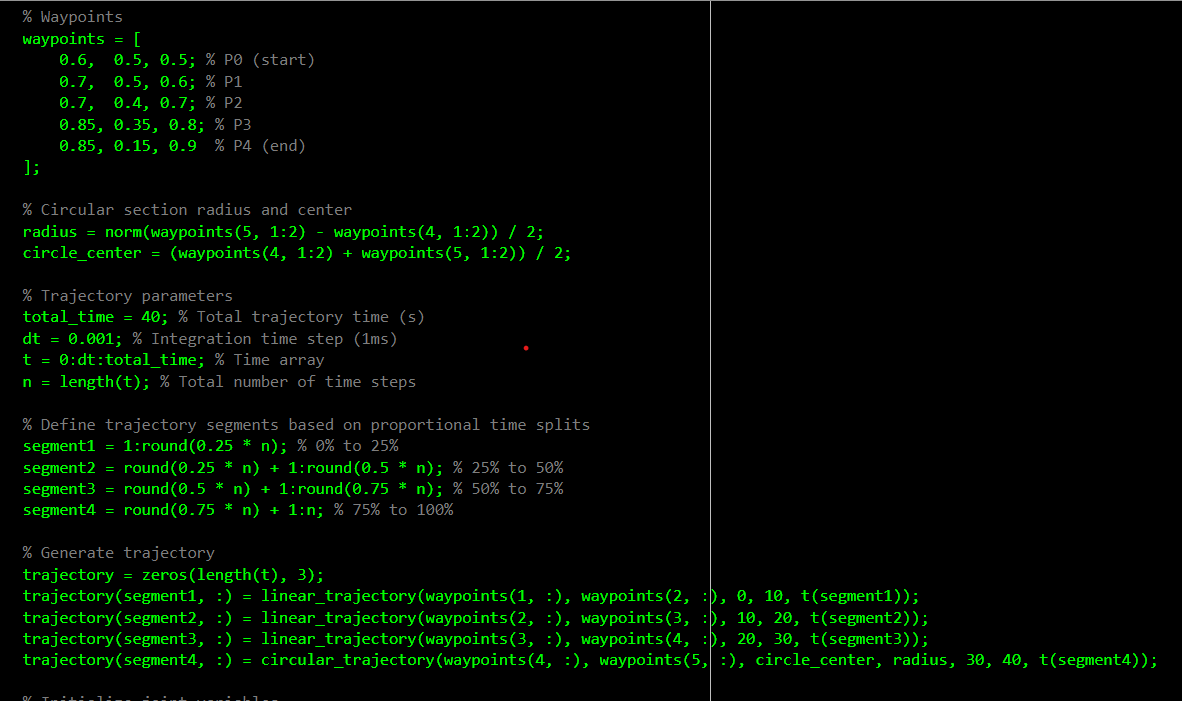
\includegraphics[scale = 0.72]{C1}
		\includegraphics[scale = 0.73]{C2}
		\\
		\includegraphics[scale = 0.72]{C3}
		\\
		\includegraphics[scale = 0.71]{C4}
		
			\subsubsection{Results}
		\begin{figure}[H]
			\centering
			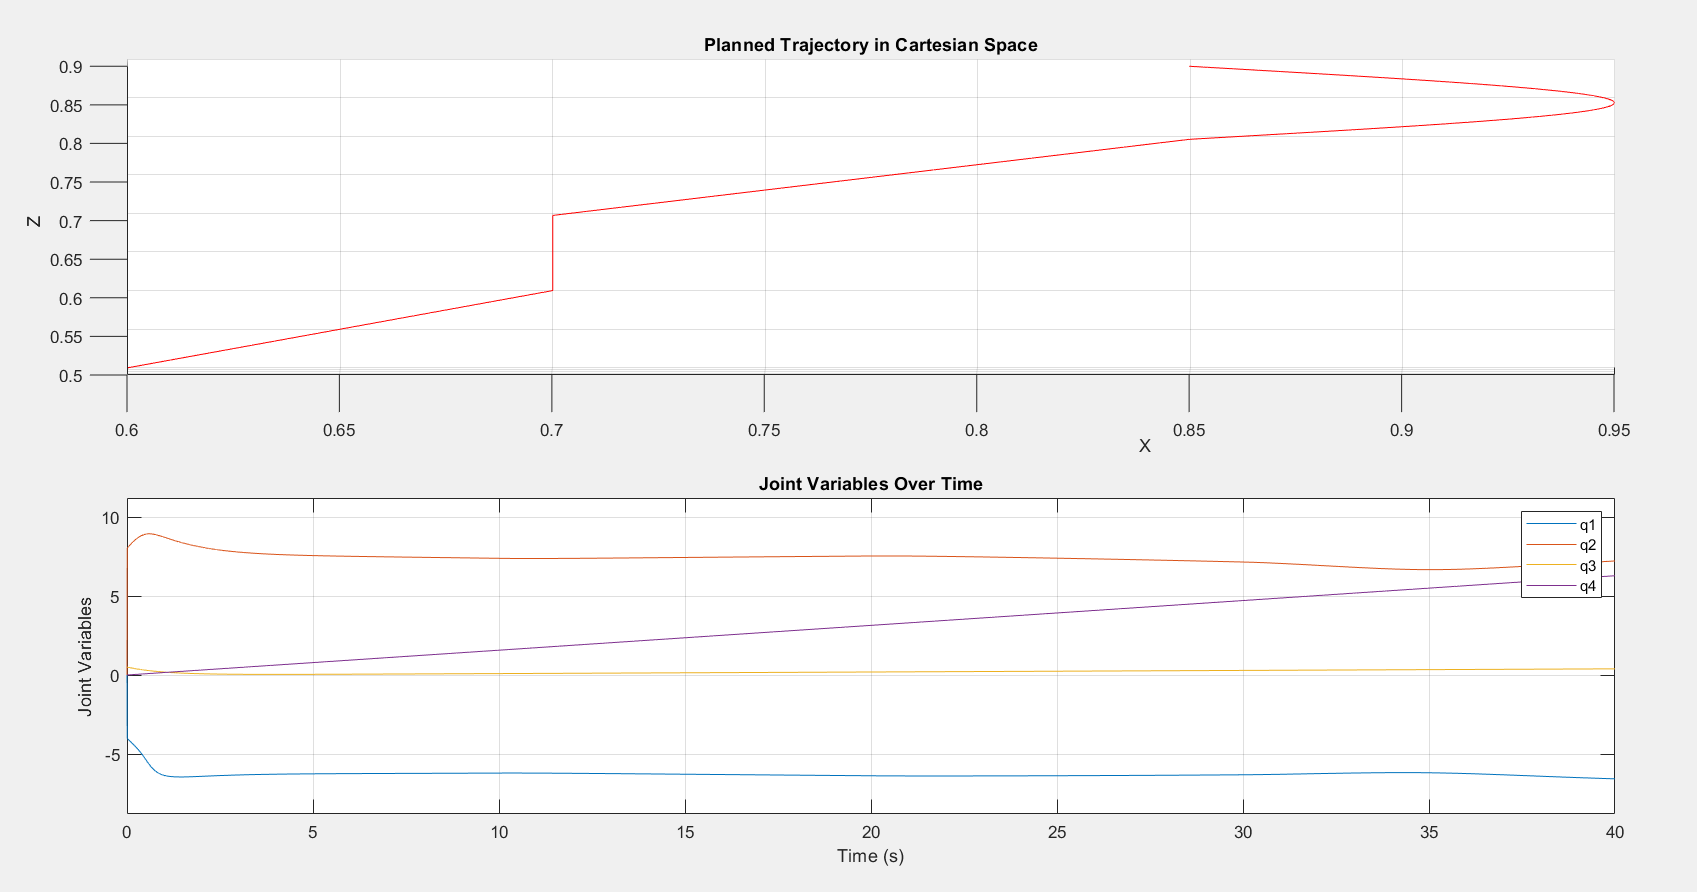
\includegraphics[scale=0.5]{R7} % Adjust the file path and scale as needed
			\caption{Kinematic Inversion using Inverse Jacobian Method 1}
			\label{run10} % Add a label for referencing this figure
		\end{figure}
		\begin{figure}[H]
			\centering
			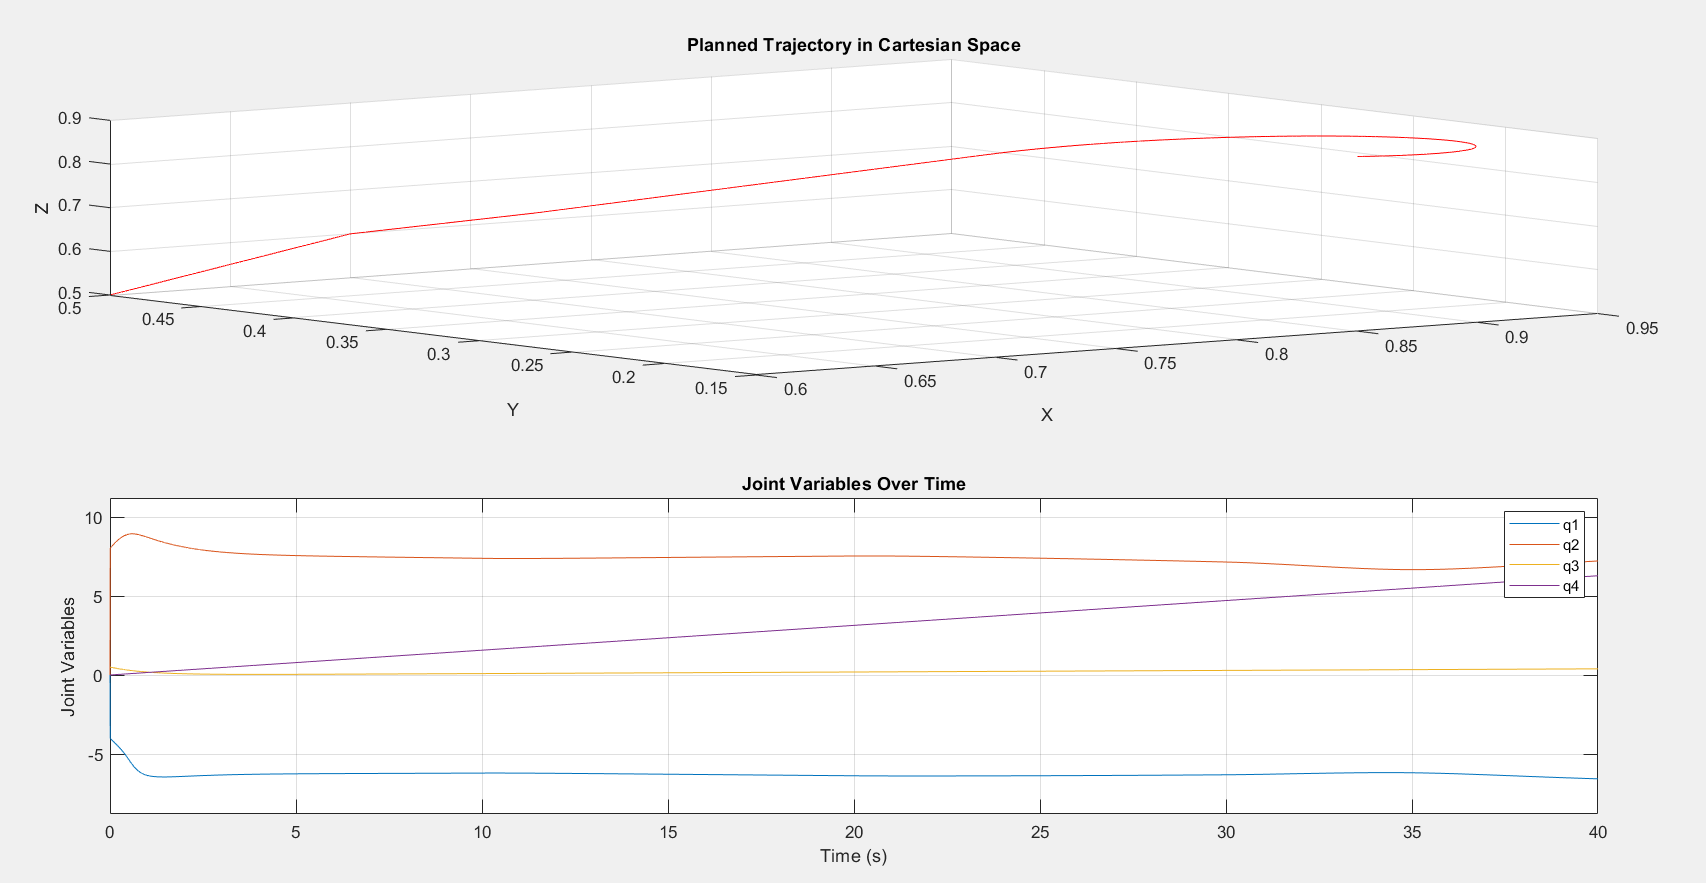
\includegraphics[scale=0.5]{R5} % Adjust the file path and scale as needed
			\caption{Kinematic Inversion using Inverse Jacobian Method 2}
			\label{run} % Add a label for referencing this figure
		\end{figure}
		\subsection{Transpose Jacobian}
			Transpose Jacobian method for kinematic inversion, is an alternative to the inverse Jacobian method. It is particularly useful when computational simplicity is preferred or when a direct inverse of the Jacobian is not feasible.
		
		
	
		
	\subsubsection{Code Implementation}
		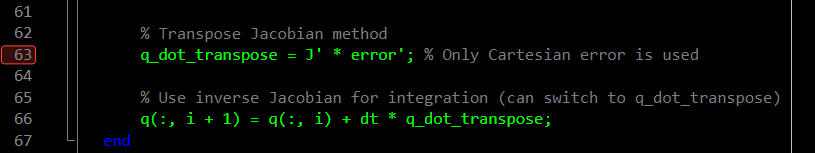
\includegraphics[scale = 1]{TR1}
	
		1. Error Computation:
		\\The error vector (\(\mathbf{e}\)) is computed as the difference between the desired and current end-effector positions in Cartesian space:
		\begin{equation}
		\mathbf{e} = [x_{\text{desired}} - x_{\text{current}}, \, y_{\text{desired}} - y_{\text{current}}, \, z_{\text{desired}} - z_{\text{current}}]^T.
		\end{equation}
		2. Joint Velocity Calculation:\\The transpose of the Jacobian (\(J^T\)) is multiplied by the error vector to compute the joint velocities (\(\dot{\mathbf{q}}\))
		. In matlab:
		\begin{center}
			\texttt{q\_dot\_transpose = J' * error';}
		\end{center}
		
		The transpose Jacobian essentially distributes the operational space error across the joints, guiding the robot toward the desired trajectory.\\\\3. Euler Integration:
		- The joint variables are updated using the Euler integration rule:
		\begin{equation}
			\mathbf{q}(t + \Delta t) = \mathbf{q}(t) + \Delta t \, \dot{\mathbf{q}}.
		\end{equation}
		
		In the code:
	\begin{center}
		\texttt{q(:, i + 1) = q(:, i) + dt * q\_dot\_transpose;}
	\end{center}
	\subsubsection{Results}
		\begin{figure}[H]
		\centering
		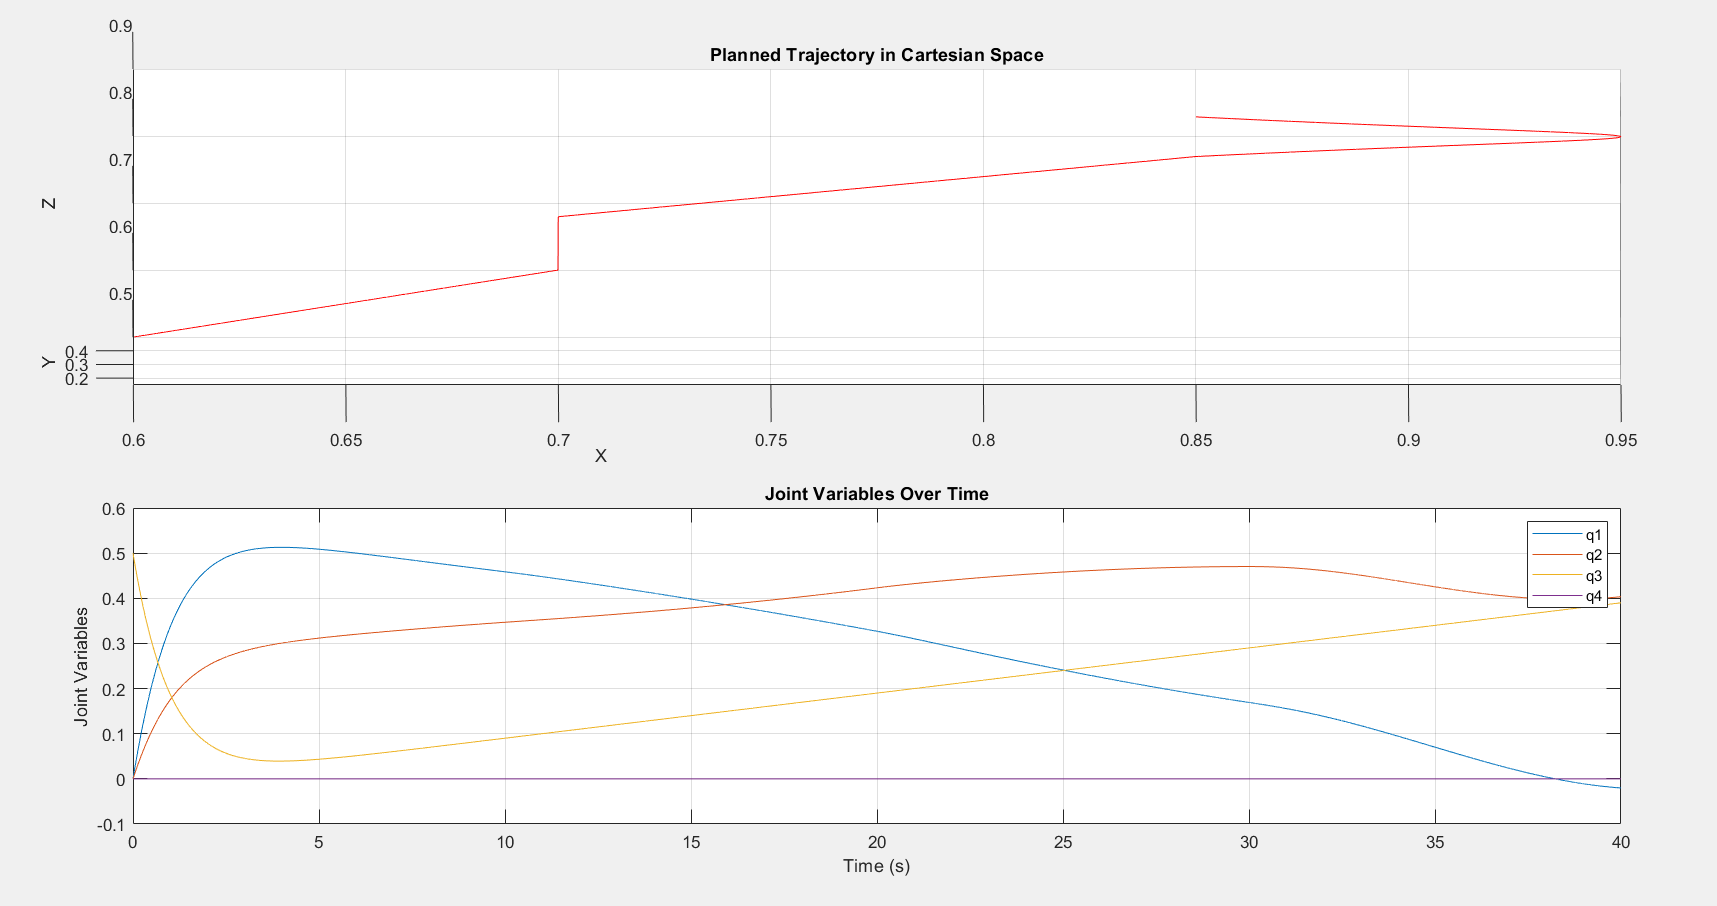
\includegraphics[scale=0.5]{R1} % Adjust the file path and scale as needed
		\caption{Kinematic Inversion using Jacobian Transpose Method 1}
		\label{run10} % Add a label for referencing this figure
	\end{figure}
	\begin{figure}[H]
		\centering
		\includegraphics[scale=0.5]{D5} % Adjust the file path and scale as needed
		\caption{Kinematic Inversion using Jacobian Transpose Method 2}
		\label{run10} % Add a label for referencing this figure
	\end{figure}
	\subsection{Key Considerations in the Code}
	Switching Between Methods:\\The code includes a flexible structure to switch between the transpose Jacobian and the inverse.
			\begin{figure}[H]
			\centering
			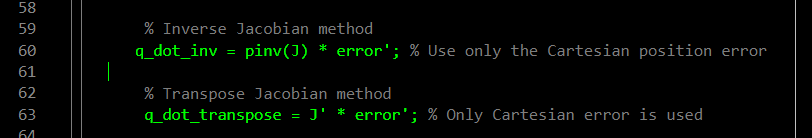
\includegraphics[scale=1.01]{D1} % Adjust the file path and scale as needed
			\caption{Code for Tranpose and Inverse Jacobian}
			\label{run10} % Add a label for referencing this figure
		\end{figure}
		This modularity allows for comparative analysis of the two approaches.
		
		\subsection{Simulink Models}
			\begin{figure}[H]
			\centering
			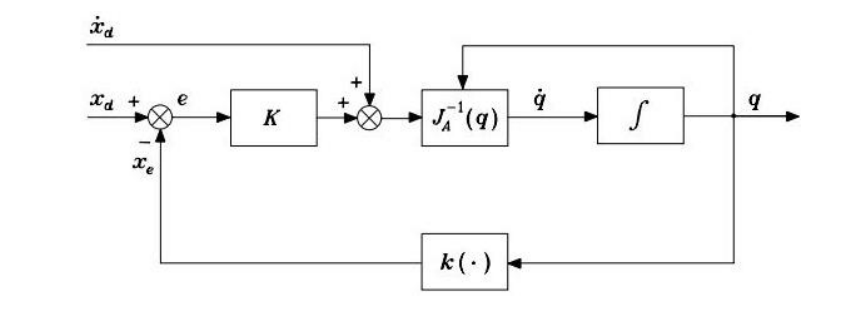
\includegraphics[scale=0.7]{S0} % Adjust the file path and scale as needed
			\caption{Control Model for Inverse Jacobian}
			\label{run10} % Add a label for referencing this figure
		\end{figure}
			\begin{figure}[H]
			\centering
			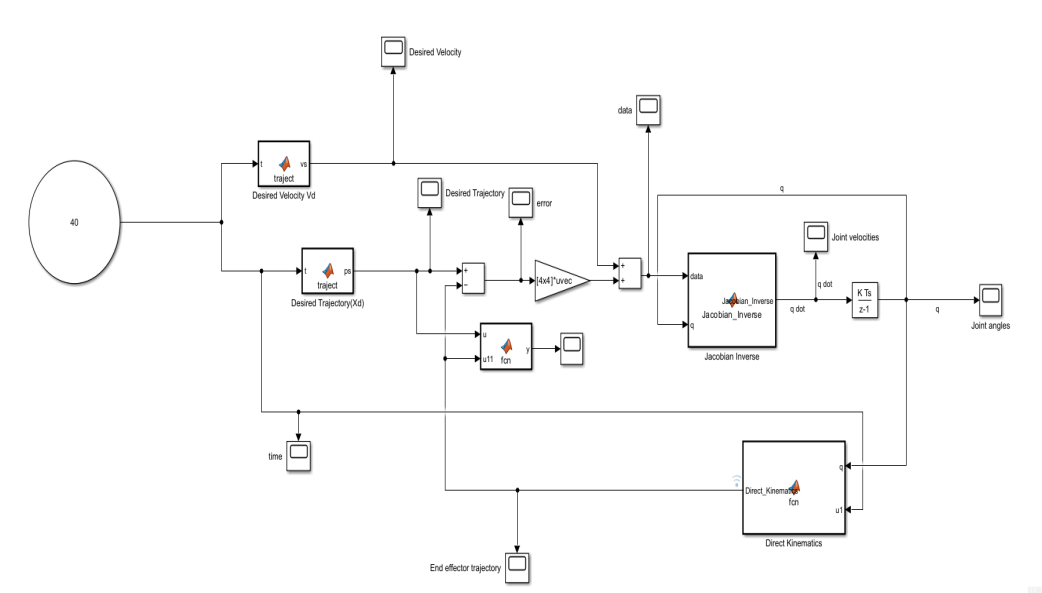
\includegraphics[scale=0.7]{S1} % Adjust the file path and scale as needed
			\caption{Simulink Model for Inverse Jacobian}
			\label{run10} % Add a label for referencing this figure
		\end{figure}
			\begin{figure}[H]
			\centering
			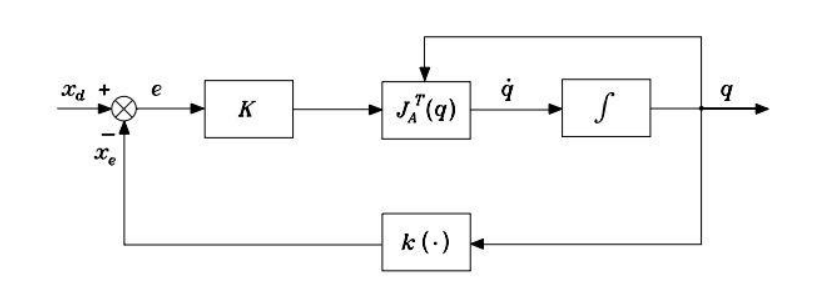
\includegraphics[scale=0.7]{S2} % Adjust the file path and scale as needed
			\caption{Control Model for Transpose of Jacobian}
			\label{run10} % Add a label for referencing this figure
		\end{figure}
		\hspace{-10mm}
			\begin{figure}[H]
			\hspace{-15mm}
			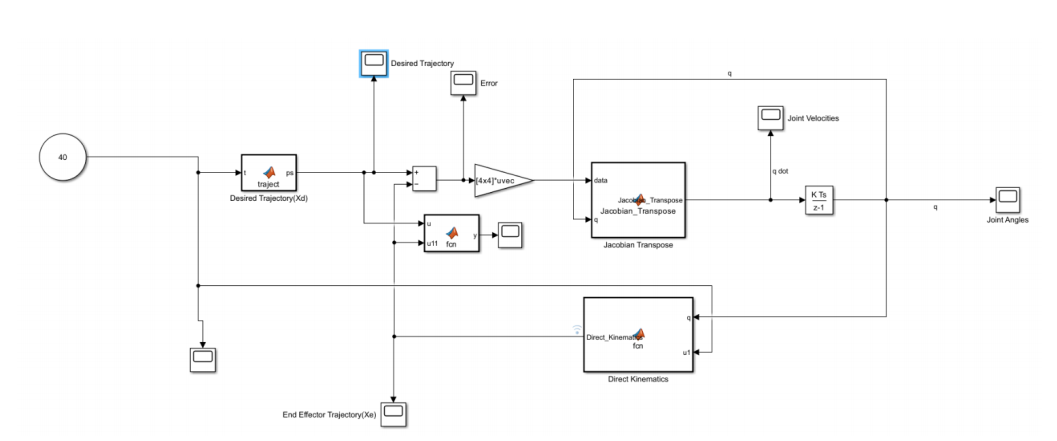
\includegraphics[scale=0.9]{S3} % Adjust the file path and scale as needed
			\caption{Simulink Model for Transpose of Jacobian}
			\label{run10} % Add a label for referencing this figure
		\end{figure}
		
		\subsection{Conclusion}
		The transpose Jacobian method provides a simple and computationally efficient way to implement kinematic inversion. While it does not guarantee optimal joint movements or exploit redundancies, it is effective for reducing the operational space error along the planned trajectory. By incorporating this method into the code, we demonstrated its practicality and versatility as an alternative to the inverse Jacobian approach.
		
	\chapter{Relaxing a Component of Operational Space}
I implemented a solution using MATLAB. The objective was to develop an algorithm that handles kinematic inversion while selectively relaxing components of the operational space based on the specified constraints. \\By "relaxing," we mean de-prioritizing or reducing the constraints on a specific operational space component, such as orientation (\(\phi\)) or height (\(z\)), allowing the robot greater freedom to optimize other parameters like avoiding joint limits or obstacles. The solution used the pseudo-inverse Jacobian to compute the required joint velocities q for tracking the trajectory while adhering to these constraints.\\The pseudo-inverse Jacobian, \(\mathbf{J}^\dagger\), was used to compute the joint velocities that minimized the error between the desired and current end-effector positions:
\[
\dot{\mathbf{q}} = \mathbf{J}^\dagger \mathbf{e}.
\]

where:\\
 \(\mathbf{e} = \mathbf{x}_{\text{desired}} - \mathbf{x}_{\text{current}}\) is the operational space error.\\
 \(\mathbf{J}^\dagger = \mathbf{J}^T (\mathbf{J} \mathbf{J}^T)^{-1}\) is the Moore-Penrose pseudo-inverse of the Jacobian.

This ensures that the end-effector accurately follows the desired trajectory.
	\addtocounter{section}{6} 
\addtocounter{subsection}{0}
\subsection{Relaxation of the Orientation Component (\(\phi\))}
When relaxing \(\phi\), the error and Jacobian contributions for the rotational component were removed. This allowed the robot to prioritize avoiding joint limits over maintaining a specific orientation:

\begin{center}
	\texttt{\% Relax the orientation component (phi) \\
		J(:, 4) = 0; \% Remove the contribution of phi from the Jacobian}
\end{center}

\subsection{Relaxation of the \(z\)-Component}
When relaxing \(z\), the error in the height component was set to zero, allowing the end-effector to adjust its \(z\)-position freely to maximize the distance from obstacles:
```matlab
% Relax the z-component
error(3) = 0; % Remove the constraint on z in the operational space
```

\subsection{Maximizing the Distance from Joint Limits}
To ensure the robot stayed far from its joint limits, we incorporated a weighting term into the pseudo-inverse calculation. This penalized configurations near the joint limits:

\begin{center}
	\texttt{
		q\_center = 0.5 * (q\_min + q\_max); \% Midpoint of joint limits \\
		q\_range = q\_max - q\_min; \% Range of joint limits \\
		weight = diag(1 ./ (q\_range - abs(q(:, i) - q\_center)).\^{}2); \% Weight matrix \\
		q\_dot = pinv(J * weight) * error'; \% Weighted pseudo-inverse
	}
\end{center}


\subsection{Incorporating Obstacles}
The obstacle is modelled as a circle in the workspace.
\begin{center}
	\texttt{
		 \% Obstacle\_parameters \\obstacle\_position = [0.75, 0.3, 0.75]; % Location of the obstacle
		\\obstacle\_radius = 0.5; % Radius of the obstacle
		\hspace{0.5cm} 
	}
\end{center}
For obstacle avoidance, we defined a repulsive potential field around the obstacle. The \(z\)-component relaxation allowed the robot to adjust its height to avoid collisions.

\begin{center}
	\texttt{
		\% Introduce obstacle avoidance \\
		if norm(p\_current - obstacle\_position) < obstacle\_radius \\
		\hspace{0.5cm} error(3) = 0; \% Relax z to avoid obstacle \\}
\end{center}






\subsection{Code}
\begin{figure}[H]
	\hspace{-15mm}
	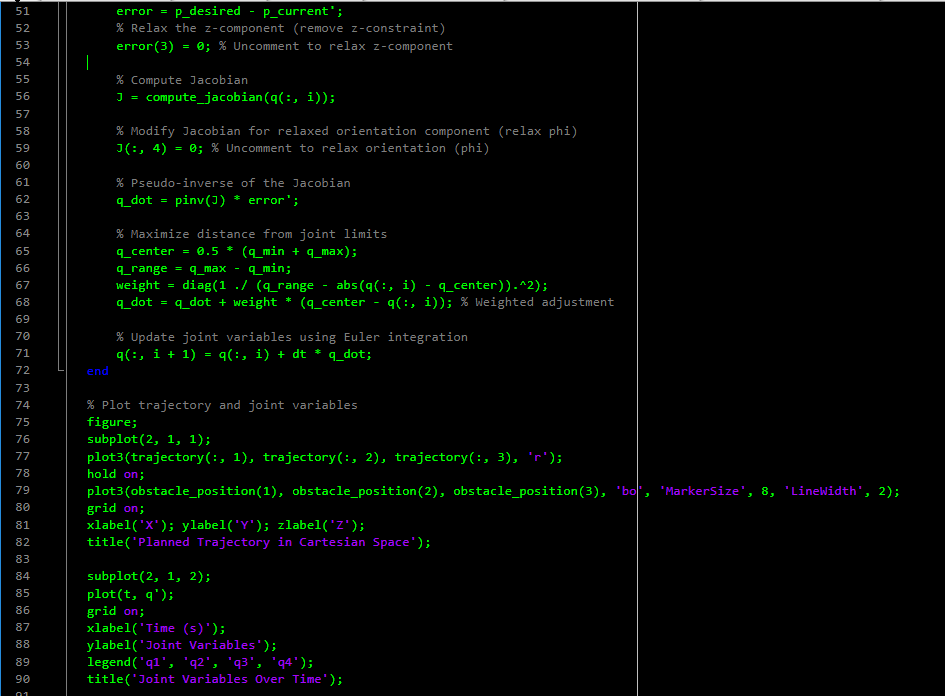
\includegraphics[scale=1]{LC} % Adjust the file path and scale as needed
	\caption{Chapter 6 Code}
	\label{run10} % Add a label for referencing this figure
\end{figure}
\subsection{Results}
The blue dot in the graph below is the obstacle.
\begin{figure}[H]
	\hspace{-15mm}
	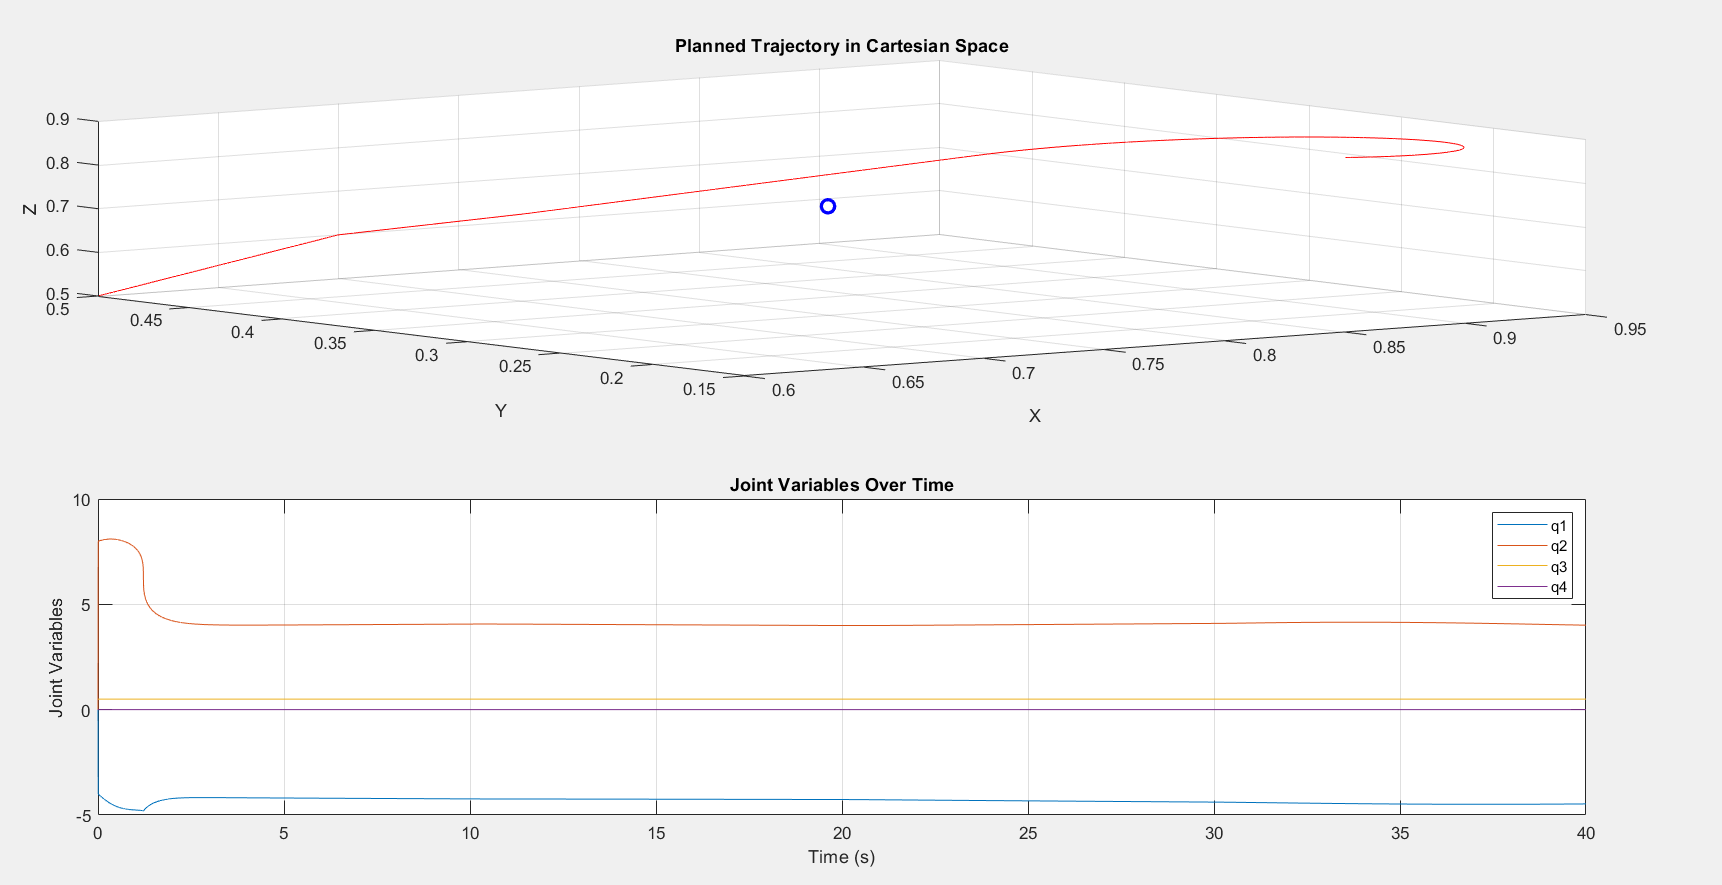
\includegraphics[scale=0.56]{R8} % Adjust the file path and scale as needed
	\caption{Relaxed phi}
	\label{run10} % Add a label for referencing this figure
\end{figure}
\begin{figure}[H]
	\hspace{-15mm}
	\includegraphics[scale=0.56]{R9} % Adjust the file path and scale as needed
	\caption{Relaxed Z}
	\label{run10} % Add a label for referencing this figure
\end{figure}
\subsection{Observations}
1. Relaxing Orientation (\(\phi\)):\\a. Allowed the robot to focus on maintaining distance from joint limits.\\b. Orientation was left uncontrolled, providing flexibility in movement.\\\\2. Relaxing \(z\)-Component:\\a. Enabled the robot to vary its height dynamically to avoid collisions.\\b. Sacrificed precise \(z\)-position control for obstacle avoidance.\\\\3. Joint Limit Avoidance:\\The weighting ensured that joint velocities moved the configuration away from boundaries, increasing safety and operational range.

\subsection{Simulink Model}
\begin{figure}[H]
	\hspace{-15mm}
	\includegraphics[scale=0.9]{S5} % Adjust the file path and scale as needed
	\caption{Simulink Model of the relaxed phi}
	\label{run10} % Add a label for referencing this figure
\end{figure}
\begin{figure}[H]
	\hspace{-15mm}
	\includegraphics[scale=0.8]{S6} % Adjust the file path and scale as needed
	\caption{Simulink Model of the relaxed Z}
	\label{run10} % Add a label for referencing this figure
\end{figure}
\subsection{Conclusion}

By implementing the pseudo-inverse Jacobian method and strategically relaxing operational space components, we achieved a robust and flexible algorithm for trajectory tracking. Relaxing \(\phi\) or \(z\) provided the robot with additional degrees of freedom to optimize performance in specific scenarios, such as maximizing distance from joint limits or avoiding obstacles. These techniques highlight the importance of balancing constraints and priorities in robotic trajectory planning.
	
		\chapter*{References}
		\addcontentsline{toc}{chapter}{References}

		\begin{enumerate}
			\item \textit{Robotics Modelling, Planning and Control}, by Bruno Siciliano, Lorenzo Sciavicco, Luigi Villani, Giuseppe Oriolo.
			\item \textit{Robotics Toolbox Guide} by Peter Corke.
		\end{enumerate}
		

		
\end{document}
